% Chapter 1
\chapter{Resultados} % Main chapter title
\label{Cap_Res} % For referencing the chapter elsewhere, use \ref{Chapter1} 

Para el análisis de los resultados obtenidos, se utilizaron tanto pruebas estadísticas bayesianas como pruebas clásicas o frecuentistas. En el presente apartado se presentan únicamente los resultados de los análisis bayesianos, mientras que los resultados de los análisis clásicos se incluyen en los Apéndices. En general, ambas aproximaciones apuntan hacia las mismas conclusiones.\\

\section{Análisis Bayesiano}\\

Se decidió presentar los resultados del análisis bayesiano porque se considera que el factor de Bayes, que funciona como una alternativa al \textit{p-value} como medida de significancia estadística, refleja de forma mucho más clara la  relación entre los datos obtenidos y las hipótesis nula y alternativa, al señalar cuántas veces es más probable que la evidencia haya sido producida bajo la hipótesis alterna respecto a la hipótesis nula ($BF_{10}$), o viceversa ($BF_{01}$).\\

\section{Consistencia entre creencias y elecciones en el primer subjuego}\\

El primer subjuego del presente experimento presenta una replicación parcial del experimento de Lahav (\citeyear{Lahav}). En ambos casos se juega p-beauty contest por varios periodos y se utiliza un método para explicitar creencias. Las diferencias radican en el número de jugadores que participan en un periodo (3 en el presente experimento, y hasta 20 en el de Lahav), la cantidad de periodos jugados (4 en el presente experimento y 5 en el de Lahav), y el método utilizado para explicitar las creencias (en el presente experimento se preguntó directamente por el número que se creía elegirían los otros jugadores, mientras que en el experimento de Lahav se estimaba el número de jugadores que elegirían un número dentro de ciertos rangos).\\

\begin{figure}[hp]
\centering
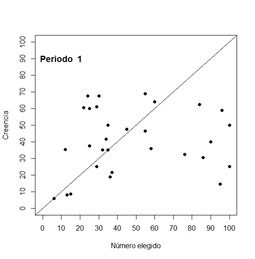
\includegraphics[width=0.45\textwidth]{Figures/F1_1} & 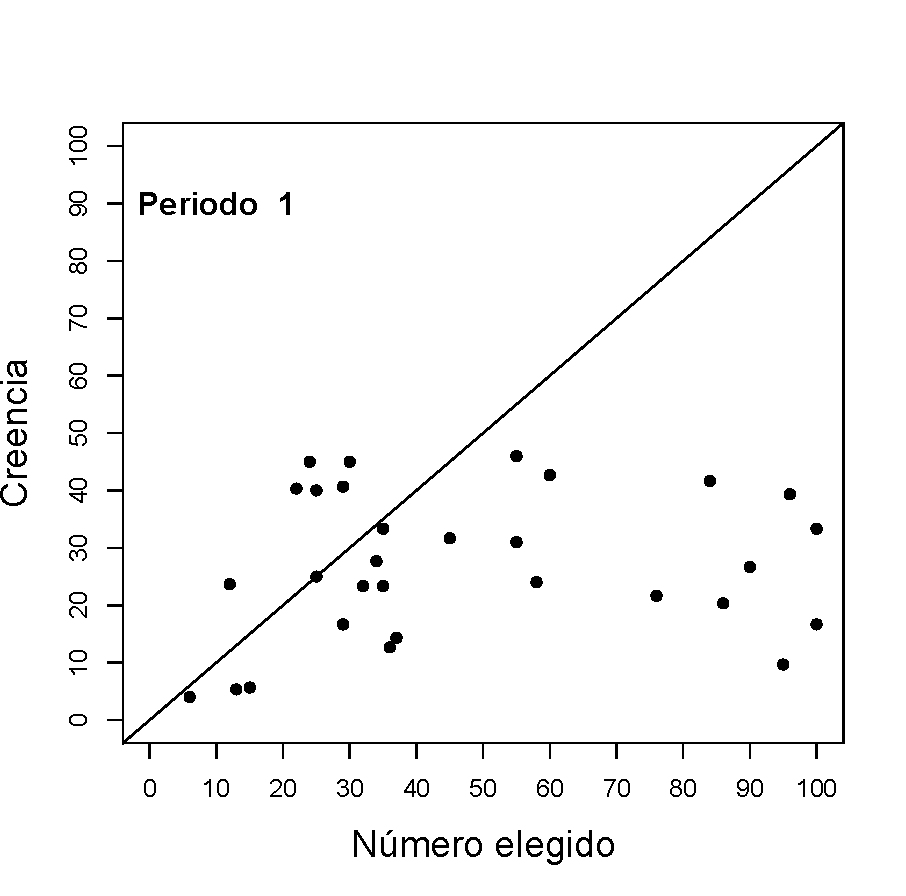
\includegraphics[width=0.45\textwidth]{Figures/F1_2} 
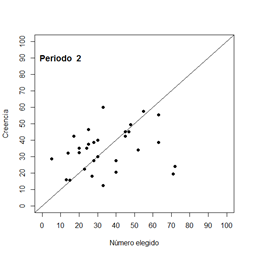
\includegraphics[width=0.45\textwidth]{Figures/F1_3} & 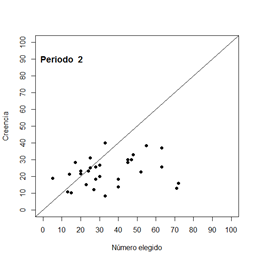
\includegraphics[width=0.45\textwidth]{Figures/F1_4} 
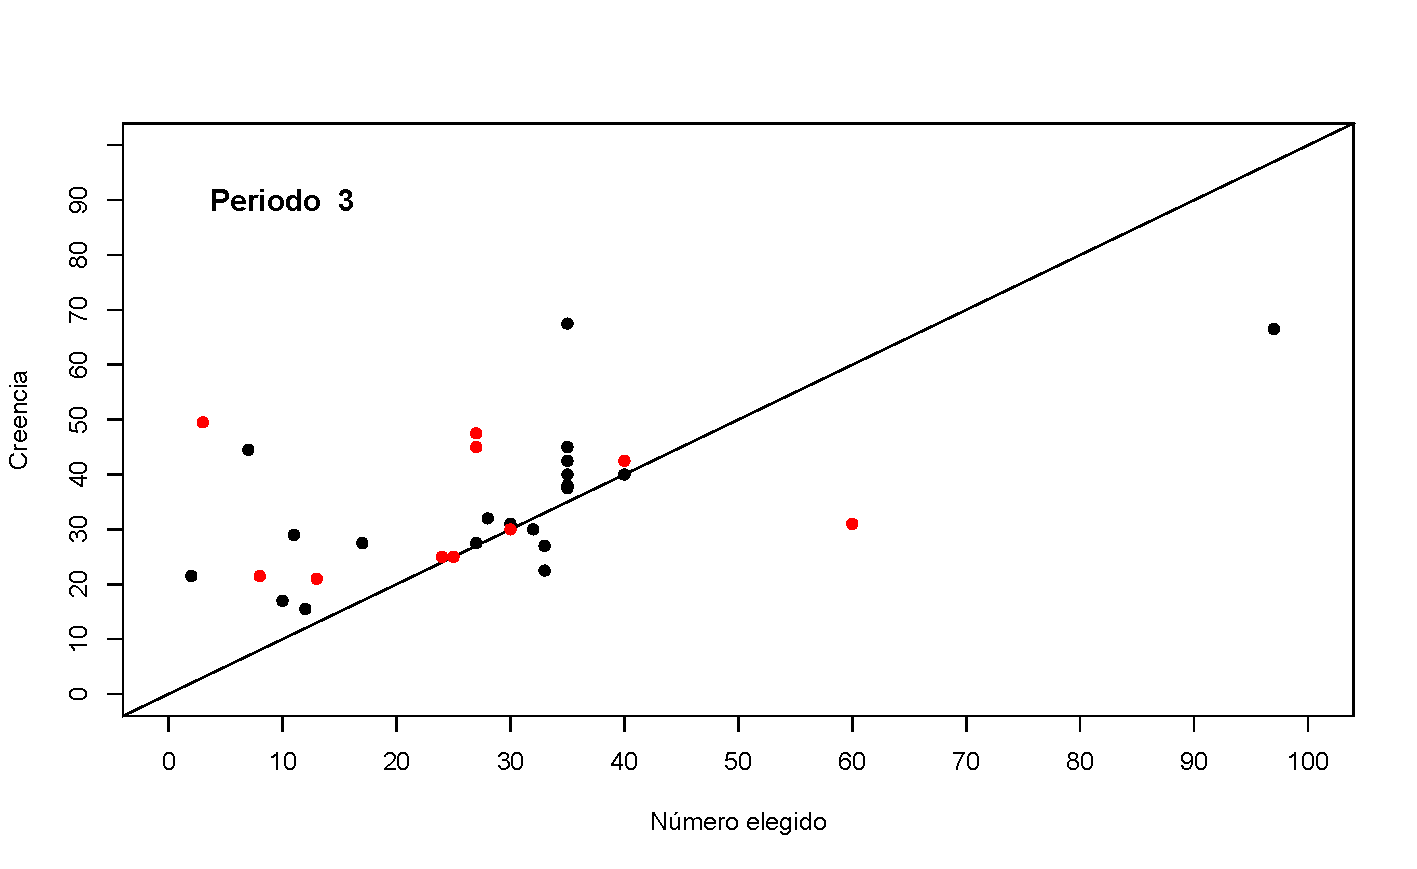
\includegraphics[width=0.45\textwidth]{Figures/F1_5} & 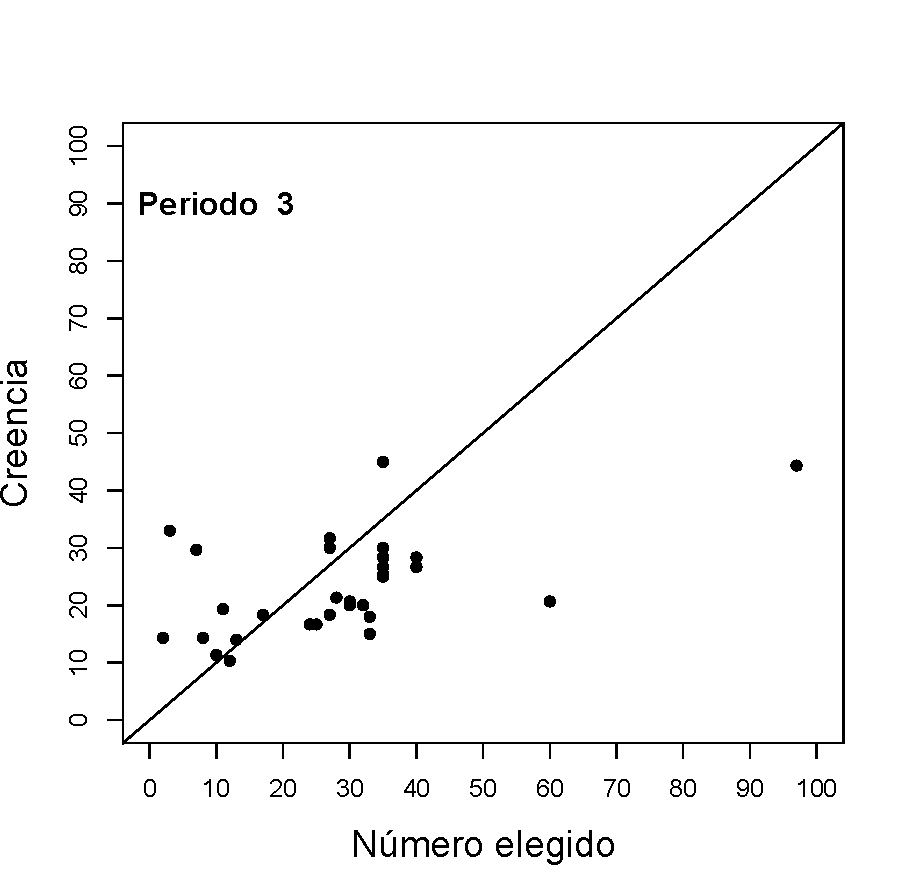
\includegraphics[width=0.45\textwidth]{Figures/F1_6} 
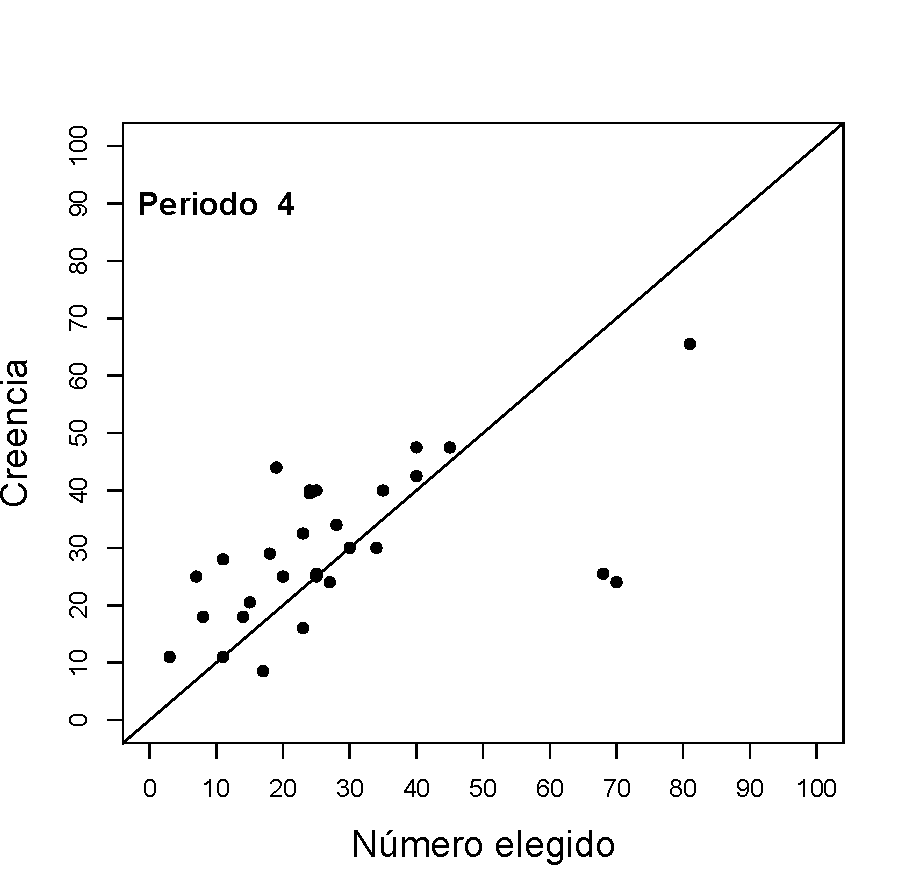
\includegraphics[width=0.45\textwidth]{Figures/F1_7} & 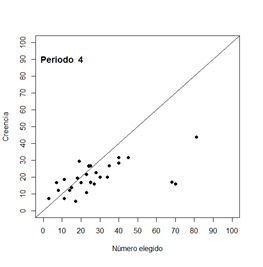
\includegraphics[width=0.45\textwidth]{Figures/F1_8} 
\decoRule
\caption[Exploración visual de la consistencia entre creencias y elecciones]{Comparación entre los números elegoidos por los participantes y el promedio de las creencias registradas. Los puntos más cercanos a la línea de identidad señalan una mayor consistencia. En las figuras del lado izquierdo las creencias promedio son multiplicadas por $p$ y en el lado derecho se omite dicha operación.}
\label{fig:Consistencia}
\end{figure}

En la Figura~\ref{fig:Consistencia} se contrasta la elección de cada participante con el promedio de las creencias registradas para cada uno de los periodos del Subjuego 1, tomando en cuenta la multiplicación por $p$ de éstas y omitiéndola (paneles izquierdos y derechos, respectivamente). Se observa que en ambos casos la diferencia entre creencias y elecciones se reduce periodo a periodo, pues en periodos posteriores los puntos se acercan más a la línea de identidad. Sin embargo, como ya se ha mencionado, esto puede deberse únicamente a que los valores elegidos se acercan más al límite inferior del espacio de elección.\\

Para evaluar la consistencia entre las creencias de los participantes y sus números elegidos tomando en cuenta el efecto de suelo, se emplearon dos métodos: el primero de ellos, computa la \textit{Diferencia Normalizada} entre las creencias y las elecciones de los participantes de acuerdo con las elecciones promedio observadas en cada periodo (Lahav, \citeyear{2015}); el segundo, calcula la \textit{Diferencia Relativa} entre creencias y elecciones a partir del punto medio entre ambos valores (método empleado por Slonim, \citeyear{Slonim}, para calcular el cambio relativo de los números elegidos por los jugadores de un periodo al siguiente). A su vez, tal y como lo reporta Lahav, estos métodos fueron aplicados con dos variantes para evaluar el cómputo realizado por los participantes, incluyendo u omitiendo la multiplicación por el parámetro $p$.\\

El procedimiento sugerido por Lahav (\citeyear{Lahav}) para calcular las diferencias normalizadas entre las creencias y las elecciones de cada participante en cada periodo, fue incorporado a partir de la siguiente ecuación:\\

\begin{center}
$DN_i^t =  \frac{(\frac{2}{3}B_i^t - C_i^t)}{\overline{C}_t} $
\end{center}

Donde $DN_i^t$ es la Diferencia Normalizada entre las creencias y elecciones de cada participante $i$ en el periodo $t$, computada a partir de la diferencia entre  la media de los números que el participante $i$ estimó que elegirían los otros dos jugadores en el periodo $t$ multiplicado por $\frac{2}{3}$, ($\frac{2}{3}B_i^t$) y el número elegido por el propio participante $i$ para ese periodo $t$ ($C_i^t$), dividida por el promedio de los números elegidos por todos los participantes en el periodo $t$ ($\overline{C}_t$).\\

Una vez computadas las diferencias por cada participante y periodo, se calculó el promedio de las mismas para poder someterlas a un análisis estadístico que permitiera evaluar si estas fueron significativamente diferentes de 0. Para ello, se realizaron pruebas-T bayesianas de una sola muestra para cada periodo de juego. En la Tabla~\ref{DN-S1-B} se reportan los Factores de Bayes obtenidos en dicho análisis, que permiten estimar qué tantas veces es más probable que la evidencia corresponda con la Hipótesis Alterna (''¿hay diferencia entre creencias y elecciones'') respecto a la Hipótesis Nula (''no hay diferencia entre creencia y elecciones''). Como puede verse, sólamente se encontraron diferencias significativas entre creencias y elecciones en los primeros dos periodos del juego.\\

\begin{table}[h]
\caption[Diferencias Normalizadas en el Subjuego 1 (prueba t de una muestra)]{\textbf{Diferencias Normalizadas en el Subjuego 1} Prueba t bayesiana de una sola muestra que compara contra 0 el promedio de las Diferencias Normalizadas entre las creencias y las elecciones de los jugadores en cada periodo del Subjuego 1.}
\label{DN-S1-B}
\centering
\begin{tabular}{l | c c | c}
\toprule
%\tabhead{Groups} & \tabhead{Treatment X} & \tabhead{Treatment Y} \\
\textbf{} & \textbf{$BF_{10}$} & \textbf{$error\%$} & \textbf{Diferencia promedio}\\
\midrule
Periodo 1 & 19.300 & 1.823e^-6 & -0.366\\
Periodo 2 & 34.545 & 3.137e^-4 & -0.342\\
Periodo 3 & 0.281 & 2.840e^-5 & -0.097\\
Periodo 4 & 0.652 & 0.015 & -0.147\\
\bottomrule
\end{tabular}
\end{table}

En la Figura~\ref{fig:DN_S1} se presenta de manera gráfica la relación entre las distribuciones prior y posterior computadas en cada periodo. Las distribuciones prior representan la Hipótesis Nula (asume diferencias  cercanas a 0) y las distribuciones posteriores presentan la magnitud de la diferencia estimada a la luz de los datos. La forma más sencilla de interpretar estas figuras es como una razón de densidades de probabilidad: si la densidad de probabilidad es mayor en la distribución prior que en la distribución posterior en el punto de ''no diferencias'' (que señala un tamaño del efecto 0, $\delta = 0$), quiere decir que la evidencia favorece la hipótesis alterna, ya que a la luz de la evidencia es ''\textit{muy poco probable}'' (menos de lo que se esperaba de acuerdo a la distribución prior) que el tamaño de efecto tenga un valor cercano a 0.\\
  
\begin{figure}[hp]
\centering
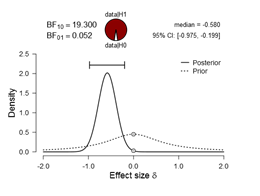
\includegraphics[width=0.45\textwidth]{Figures/F2_1} & 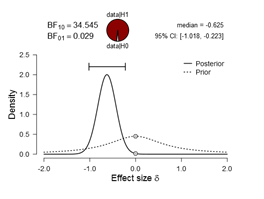
\includegraphics[width=0.45\textwidth]{Figures/F2_2} 
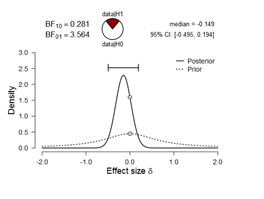
\includegraphics[width=0.45\textwidth]{Figures/F2_3} & 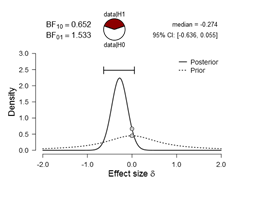
\includegraphics[width=0.45\textwidth]{Figures/F2_4} 
\decoRule
\caption[Diferencias Normalizadas entre creencias y elecciones en el Subjuegoo 1 (Factor de Bayes)]{Para la evaluación con pruebas t de una muestra de las Diferencias Normalizadas entre las creencias y las elecciones registradas en los cuatro periodos del Subjuego 1, se presenta la relación entre las distribuciones prior y posteriores computadas por cada periodo. La razón de probabilidad entre estas distribuciones en el punto $\delta = 0$ señala qué tan probable es que no hayan diferencias según los datos recabados (la distribución posterior), en comparación con la hipótesis nula (la distribución prior).}
\label{fig:DN_S1}
\end{figure}

Estos resultados son consistentes con lo que reporta Lahav (\citeyear{Lahav}): en los primeros periodos no hay consistencia entre las creencias y elecciones, pero ésta parece adquirirse conforme avanzan los periodos. Así mismo, en todos los periodos se encontraron diferencias negativas, sugiriendo que en promedio las creencias de los participantes estuvieron por debajo de sus elecciones reales.\\

En el estudio presentado por Lahav (\citeyear{Lahav}), el cómputo de la Diferencia Normalizada entre las creencias y las elecciones se realizó también omitiendo la multiplicación de las creencias por $p$, en un intento por evaluar la posibilidad de que las inconsistencias halladas entre éstas y las elecciones se deban a que los participantes no habían considerado dicha operación. El presente trabajo también incorporó dicha variación del análisis, llevada a cabo de acuerdo a la siguiente ecuación, en la que ya no se incluye la multiplicación por $\frac{2}{3}$ en $B_i^t$:\\

\begin{center}
$DN_i^t=  \frac{(B_i^t- C_i^t)}/{\overline{C}_t}$ \\
\end{center}

Nuevamente, las diferencias promedio computadas en cada periodo asumiendo que los participantes no multiplicaron sus creencias por $p$, fueron evaluadas con pruebas-T bayesianas de una sola muestra.  Este análisis arrojó resultados inversos a los encontrados cuando la multiplicación por $p$ fue tomada en cuenta: los primeros periodos no muestran diferencias significativas y los últimos, sí.  Aunado a ello, las diferencias en los periodos 3 y 4 se vuelven positivas (indicando que las creencias cayeron por encima de las elecciones). Estos resultados se presentan en la Tabla~\ref{DNnop-S1-B}.\\


\begin{table}[h]
\caption[Diferencias Normalizadas en el Subjuego 1, omitiendo la multiplicación por $p$ (prueba t de una muestra)]{\textbf{Diferencias Normalizadas en el Subjuego 1 omitiendo la multiplicación por p:} Prueba t bayesiana de una sola muestra que compara contra 0 el promedio de las Diferencias Normalizadas entre las creencias, omitiendo la multiplicación por $p$, y las elecciones de los jugadores en cada periodo del Subjuego 1.}
\label{DNnop-S1-B}
\centering
\begin{tabular}{l | c c | c}
\toprule
%\tabhead{Groups} & \tabhead{Treatment X} & \tabhead{Treatment Y} \\
\textbf{} & \textbf{$BF_{10}$} & \textbf{$error\%$} & \textbf{Diferencia promedio}\\
\midrule
Periodo 1 & 0.207 & 0.010 & -0.049\\
Periodo 2 & 0.196 & 0.013 & -0.012\\
Periodo 3 & 3.811 & 3.017e^-5 & 0.355\\
Periodo 4 & 1.861 & 4.032e^-4 & 0.280\\
\bottomrule
\end{tabular}
\end{table}

De acuerdo con el Factor de Bayes, aunque la Hipótesis Alterna es más probable en los periodos 3 y 4 (es decir, que sí hay diferencias entre las creencias y las elecciones) respecto de la Hipótesis Nula, la evidencia acumulada es relativamente pequeña, (particularmente en el periodo 4, donde podría considerarse anecdótica). En la Figura~\ref{fig:DNnop_S1} se muestra la relación entre las distribuciones prior y posteriores de cada periodo.\\

\begin{figure}[hp]
\centering
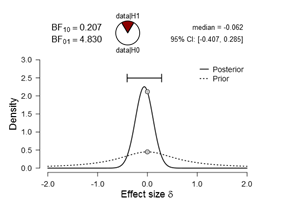
\includegraphics[width=0.45\textwidth]{Figures/F3_1} & 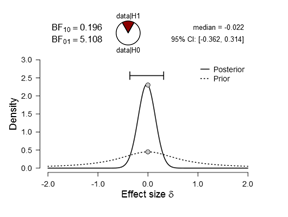
\includegraphics[width=0.45\textwidth]{Figures/F3_2} 
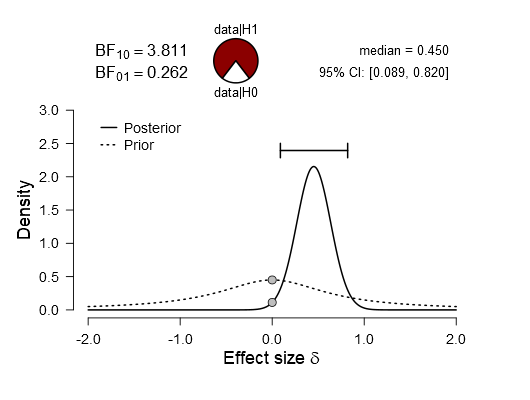
\includegraphics[width=0.45\textwidth]{Figures/F3_3} & 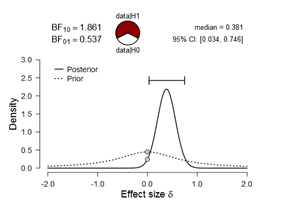
\includegraphics[width=0.45\textwidth]{Figures/F3_4} 
\decoRule
\caption[Diferencias Normalizadas entre creencias y elecciones en el Subjuegoo 1, omitiendo la multiplicación por $p$ (Factor de Bayes)]{Para la evaluación con pruebas t de una muestra de las Diferencias Normalizadas entre las creencias (omitiendo la multiplicación por $p$) y las elecciones registradas en los cuatro periodos del Subjuego 1, se ilustra la relación entre las distribuciones prior y posteriores computadas por cada periodo. La razón de probabilidades en el punto $\delta = 0$ indica qué tan probable es, a la luz de los datos (la distribución posterior), que no hayan diferencias en comparación con lo que nuestra Hipótesis Nula supondría.}
\label{fig:DNnop_S1}
\end{figure}

Este resultado difiere considerablemente de los hallazgos reportados por Lahav (\citeyear{Lahav}), quien reportó que al excluir la multiplicación por $\frac{2}{3}$, las diferencias en los cuatro periodos se volvieron positivas, significativamente diferentes de 0, y en general, más grandes que cuando la multiplicación por $p$ era tomada en cuenta. En el estudio conducido por Lahav, dichos resultados fueron interpretados como un indicador de que los participantes sí toman en cuenta la multiplicación por $p$.\\

Cuando se incluye la multiplicación por $p$ en el cálculo de las Diferencias Normalizadas entre creencias y elecciones en el presente estudio, se encuentra que éstas fueron significativas en los primeros periodo, y al excluir dicha multiplicación, las diferencias significativas aparecen sólo en los últimos periodos, aunque la evidencia parece ser débil. Estos resultados podrían estar sugiriendo a que los participantes comienzan el juego sin considerar la multiplicación por $\frac{2}{3}$, pero la incorporan en sus decisiones al avanzar en los periodos (o por lo menos, aprenden que el número objetivo siempre está por debajo del número promedio).\\

En general, a pesar de las diferencias en los métodos empleados para la elicitación de creencias, el presente estudio presenta hallazgos similares a los reportados por Lahav (\citeyear{Lahav}) al emplear el método propuesto para calcular las Diferencias Normalizadas entre las creencias y las elecciones de los participantes:\\

\begin{itemize}
\item Existen discrepancias entre las creencias y las elecciones de los participantes en los primeros periodos de juego, pero no en los últimos.\\

\item Las elecciones de los participantes suelen encontrarse entre el promedio de sus creencias respecto de los otros jugadores y el número objetivo computado de acuerdo a su multiplicación por $p$.\\
\end{itemize}

La diferencia más importante entre lo hallado en el presente estudio y lo reportado por Lahav (\citeyear{Lahav}), es que, en promedio, los participantes no parecen incorporar la multiplicación por $\frac{2}{3}$ en su elección, al menos en los primeros periodos.\\

Además de replicar el método de Diferencias Normalizadas utilizado por Lahav (\citeyear{Lahav}), las diferencias entre creencias y elecciones fueron evaluadas con un segundo método que no dependía de la elección promedio de todos los participantes en cada periodo para ponderarlas. La medida utilizada fue la Diferencia Relativa entre las creencias y elecciones de cada participante $i$ en cada periodo $t$, calculada de la siguiente manera:\\

\begin{center}
$DR_i^t =  \frac{(\frac{2}{3}B_i^t- C_i^t)}{0.5(\frac{2}{3}B_i^t + C_i^t)}$\\
\end{center}

El promedio de las Diferencias Relativas computadas por cada periodo fueron evaluadas en términos de qué tanto se alejaron de 0, mediante la realización de pruebas t bayesianas de una sola muestra, que se presentan en la Tabla~\ref{DR-S1-B}, encontrando que en tres de los cuatro periodos hubo diferencias significativas entre las creencias y elecciones. En la Figura~\ref{fig:DR_S1} se presenta la comparación entre las distribuciones prior y posterior computadas por cada periodo.\\


\begin{table}[h]
\caption[Diferencias Relativas en el Subjuego 1 (prueba t de una muestra)]{\textbf{Diferencias Relativas en el Subjuego 1} Prueba t bayesiana de una sola muestra que compara contra 0 el promedio de las Diferencias Relativas computadas entre las creencias y las elecciones de los jugadores en cada periodo del Subjuego 1.}
\label{DR-S1-B}
\centering
\begin{tabular}{l | c c | c}
\toprule
%\tabhead{Groups} & \tabhead{Treatment X} & \tabhead{Treatment Y} \\
\textbf{} & \textbf{$BF_{10}$} & \textbf{$error\%$} & \textbf{Diferencia promedio}\\
\midrule
Periodo 1 & 72.283 & 7.775e^-5 & -0.457\\
Periodo 2 & 12.797 & 2.047e^-6 & -0.328\\
Periodo 3 & 0.214 & 0.008 & -0.052\\
Periodo 4 & 1.871 & 4.022e^-6 & -0.212\\
\bottomrule
\end{tabular}
\end{table}
	


\begin{figure}[h]
\centering
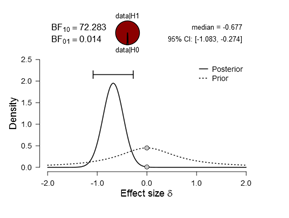
\includegraphics[width=0.45\textwidth]{Figures/F4_1} & 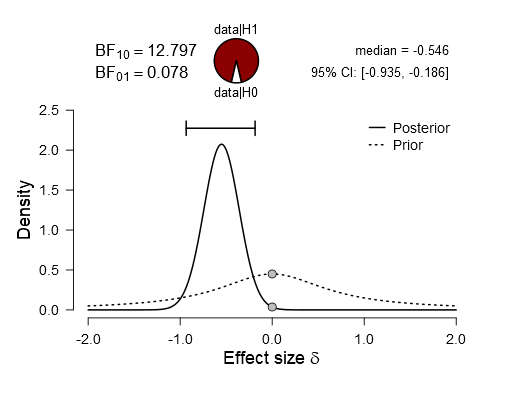
\includegraphics[width=0.45\textwidth]{Figures/F4_2} 
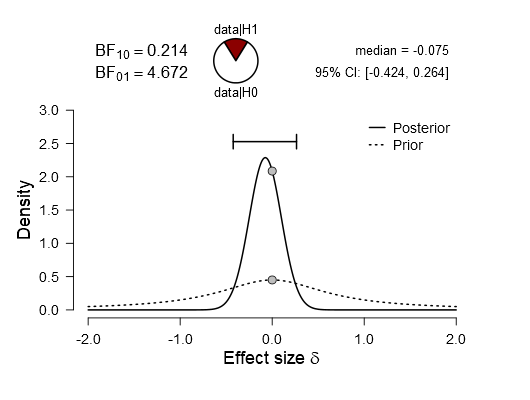
\includegraphics[width=0.45\textwidth]{Figures/F4_3} & 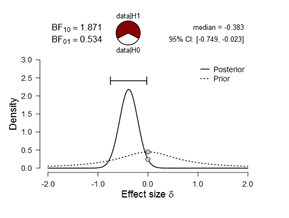
\includegraphics[width=0.45\textwidth]{Figures/F4_4} 
\decoRule
\caption[Diferencias Relativas entre creencias y elecciones en el Subjuego 1 (Factor de Bayes)]{Para la evaluación con pruebas t de una muestra de las Diferencias Relativas encontradas entre las creencias y las elecciones de los participantes a lo largo del Subjuego 1, en el punto de no diferencias, se presenta la razón de probabilidades en el punto $\delta = 0$ que indica si a la luz de los datos (la distribución posterior) es más o menos probable (y qué tanto) que no hayan diferencias entre estas, de lo que supondría la Hipótesis Nula.}
\label{fig:DR_S1}
\end{figure}

Tal y como se encontró con el método de Diferencias Normalizadas, todas las diferencias son negativas, indicando que consistentemente las creencias estuvieron por debajo de las elecciones reales. Sin embargo, contrario a lo que se esperaría con base en los resultados hallados con el método de Diferencias Normalizadas donde los participantes reducen la inconsistencia entre sus elecciones y las creencias explicitadas conforme adquieren experiencia, con el método de Diferencias Relativas se observan inconsistencias (diferencias estadísticamente significativas) entre creencias y elecciones en el periodo 4, aunque no en el periodo 3. De cualquier forma, de acuerdo con el factor de Bayes, la evidencia a favor de la hipótesis alterna en el periodo 4 es anecdótica.\\

Posteriormente, se computaron las Diferencias Relativas omitiendo la multiplicación por $p$, de acuerdo con la siguiente ecuación:\\

\begin{center}
$DR_i^t=  \frac{(B_i^t- C_i^t)}{0.5(B_i^t+ C_i^t)}$
\end{center}

Se realizaron pruebas t de una sola muestra para determinar si las Diferencias Relativas promedio en cada periodo son significativamente diferentes de 0, cuando la multiplicación por $p$ no es tomada en cuenta. En la Tabla~\ref{DRnop-S1-B} se presentan los resultados obtenidos y en la Figura~\ref{fig:DRnop_S1}, la relación entre las distribuciones prior y las posteriores en cada periodo.\\


\begin{table}[h]
\caption[Diferencias Relativas en el Subjuego 1, omitiendo la multiplicación por $p$ (prueba t de una muestra)]{\textbf{Diferencias Relativas en el Subjuego 1 omitiendo la multiplicación por p} Prueba t bayesiana de una sola muestra que compara contra 0 el promedio de las Diferencias Relativas entre las creencias y las elecciones de los jugadores en cada periodo Subjuego 1.}
\label{DRnop-S1-B}
\centering
\begin{tabular}{l | c c | c}
\toprule
%\tabhead{Groups} & \tabhead{Treatment X} & \tabhead{Treatment Y} \\
\textbf{} & \textbf{$BF_{10}$} & \textbf{$error\%$} & \textbf{Diferencia promedio}\\
\midrule
Periodo 1 & 0.269 & 5.246e^-4 & -0.101\\
Periodo 2 & 0.211 & 0.009 & 0.044\\
Periodo 3 & 8.393 & 2.307e^-6 & 0.315\\
Periodo 4 & 0.810 & 5.669e^-6 & 0.167\\
\bottomrule
\end{tabular}
\end{table}
	

\begin{figure}[h]
\centering
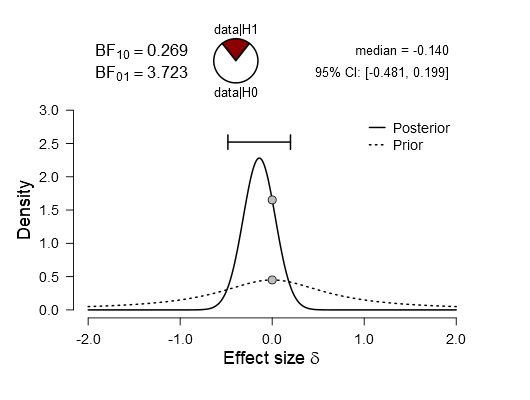
\includegraphics[width=0.45\textwidth]{Figures/F5_1} & 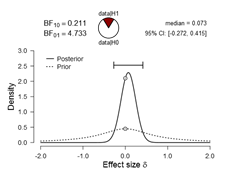
\includegraphics[width=0.45\textwidth]{Figures/F5_2} 
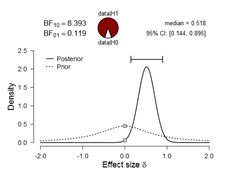
\includegraphics[width=0.45\textwidth]{Figures/F5_3} & 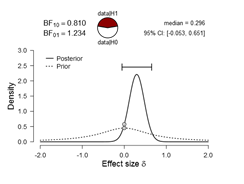
\includegraphics[width=0.45\textwidth]{Figures/F5_4} 
\decoRule
\caption[Diferencias Relativas entre creencias y elecciones en el Subjuego 1 sin la multiplicación por p (Factor de Bayes)]{Para la evaluación con pruebas t de una muestra de las Diferencias Relativas encontradas entre las creencias (sin multiplicar por $p$) y las elecciones de los participantes a lo largo del Subjuego 1, se señala la razón de probabilidades en el punto $\delta = 0$ que indica si a la luz de los datos (la distribución posterior) es más o menos probable (y qué tanto) que no hayan diferencias entre estas, de lo que supondría la Hipótesis Nula.}
\label{fig:DRnop_S1}
\end{figure}


Similar a lo observado cuando se omitió la multiplicación por $p$ en el cómputo de las Diferencias Normalizadas propuesto por Lahav (\citeyear{Lahav}), se encontró una reversión en la significancia reportada en todos los periodos, (aunque nuevamente, la evidencia en el periodo 4 es anecdótica), encontrando diferencias positivas en tres de los cuatro periodos. Esto último sugiere que con el uso del método de Diferencias Relativas, en promedio, las creencias están más cercanas y ligeramente por arriba de las elecciones reales de los participantes, cuando no se toma en cuenta la multiplicación por $p$.\\

Aunque cada uno de los dos métodos empleados para evaluar la consistencia entre las creencias y elecciones de los participantes intenta compensar la tendencia hacia el equilibrio y el problema de suelo resultante de forma diferente, ambos mostraron resultados muy similares: en los primeros periodos las diferencias entre creencias y elecciones son grandes, pero esta se reduce en los periodos posteriores, sugiriendo que los jugadores se vuelven consistentes conforme adquieren experiencia y aprenden también que para acercarse al número objetivo necesitan elegir números por debajo del promedio de sus creencias.\\

\section{Efecto de reset}\\

De acuerdo con los resultados reportados por Slonim (\citeyear{Slonim}), los jugadores presentan un efecto de '''Reset'' en la tendencia a elegir números cada vez más pequeños cuando los otros jugadores son reemplazados por jugadores nuevos, que no tienen experiencia en el juego. Tomando este hallazgo en cuenta, el presente estudio incorporó un Subjuego 2, donde sólo uno de los jugadores del Subjuego 1 permaneció jugando por otros cuatro periodos, mientras que el resto fue reemplazado por jugadores nuevos. Esta manipulación se realizó para evaluar la tendencia que en el estudio de Lahav (\citeyear{Lahav}) lleva a asumir que los jugadores se vuelven más consistentes conforme adquieren experiencia. En otras palabras, agregar un segundo Subjuego permite evaluar, con base en las respuestas del participante con experiencia, si la consistencia entre las elecciones y las creencias es algo que se adquiere con la experiencia o si es sólo el resultado del efecto de suelo asociado a la tendencia típicamente reportada en cualquier serie de juegos p-beauty contest repetido a elegir números cada vez más pequeños, (Ho, \citeyear{Teck-Hua}).\\

Para poder comparar los resultados del Subjuego 1 con el Subjuego 2, fue necesario comprobar que la incorporación de nuevos jugadores en el Subjuego 2 interrumpió la tendencia a elegir números cada vez más pequeños en los jugadores que se mantuvoerpm en el juego (los participantes A). Es decir, para corroborar que el diseño experimental propuesto permite responder a la cuestión de si las diferencias entre creencias y elecciones se reducen como reflejo de una consistencia adquirida o como producto del efecto de suelo, es necesario evaluar la presencia del efecto de Reset reportado por Slonim (\citeyear{Slonim}).\\

En la Figura~\ref{fig:Reset_cambios} se muestran los cambios en las elecciones realizadas en periodos consecutivos, por los participantes A. Los primeros tres cuadros muestran los cambios dentro del Subjuego 1 y en el cuarto panel se evalúa directamente el Efecto de Reset, al comparar la elección registrada en el último periodo del Subjuego 1 y el primer periodo del Subjuego 2. En estas gráficas, los puntos que caen por debajo de la línea de identidad indican que se eligieron números más pequeños de un periodo a otro, con lo que se observa que hay más participantes A que eligen números más pequeños entre los periodos del Subjuego 1 (por ejemplo, el $80\%$ reduce su elección entre el periodo 3 y el periodo 4), pero que esta tendencia se revierte al iniciar el subjuego 2 (el $70\%$ incrementa su número).\\

\begin{figure}[hp]
\centering
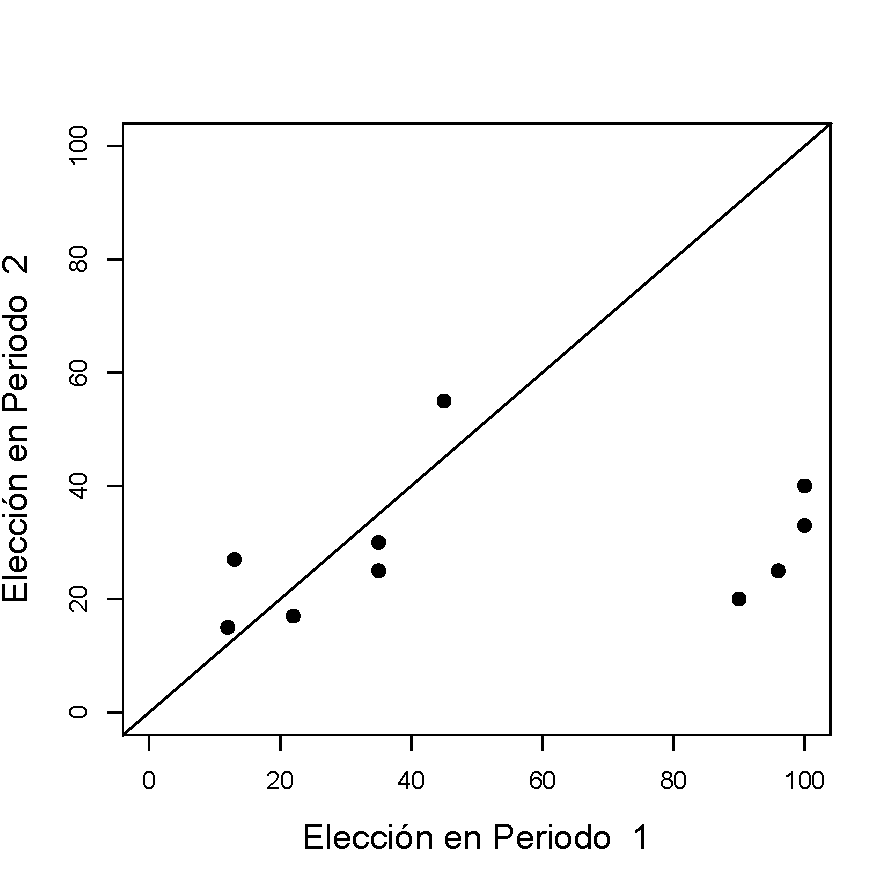
\includegraphics[width=0.45\textwidth]{Figures/F6_1} & 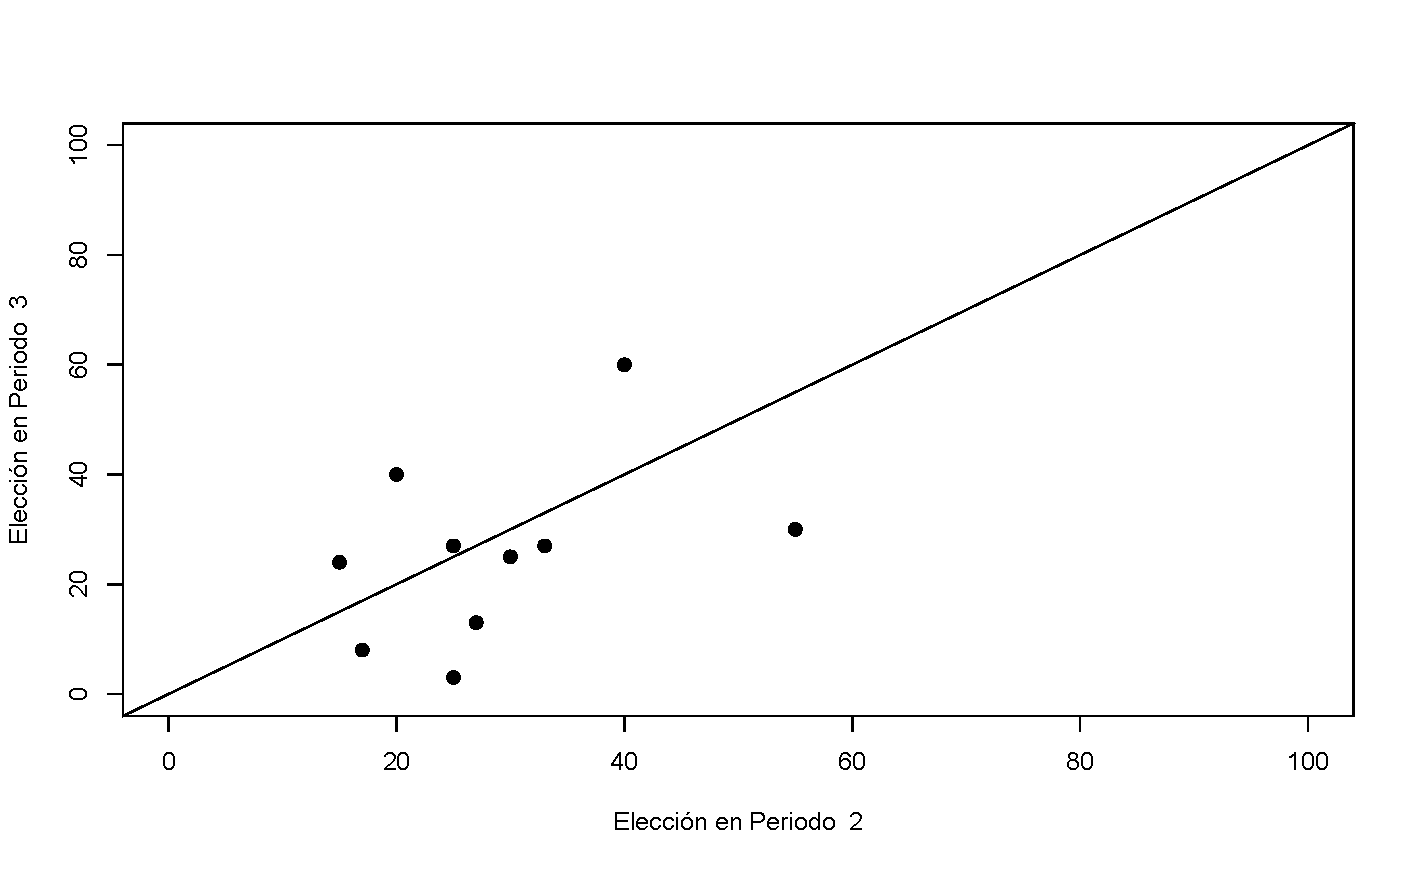
\includegraphics[width=0.45\textwidth]{Figures/F6_2} 
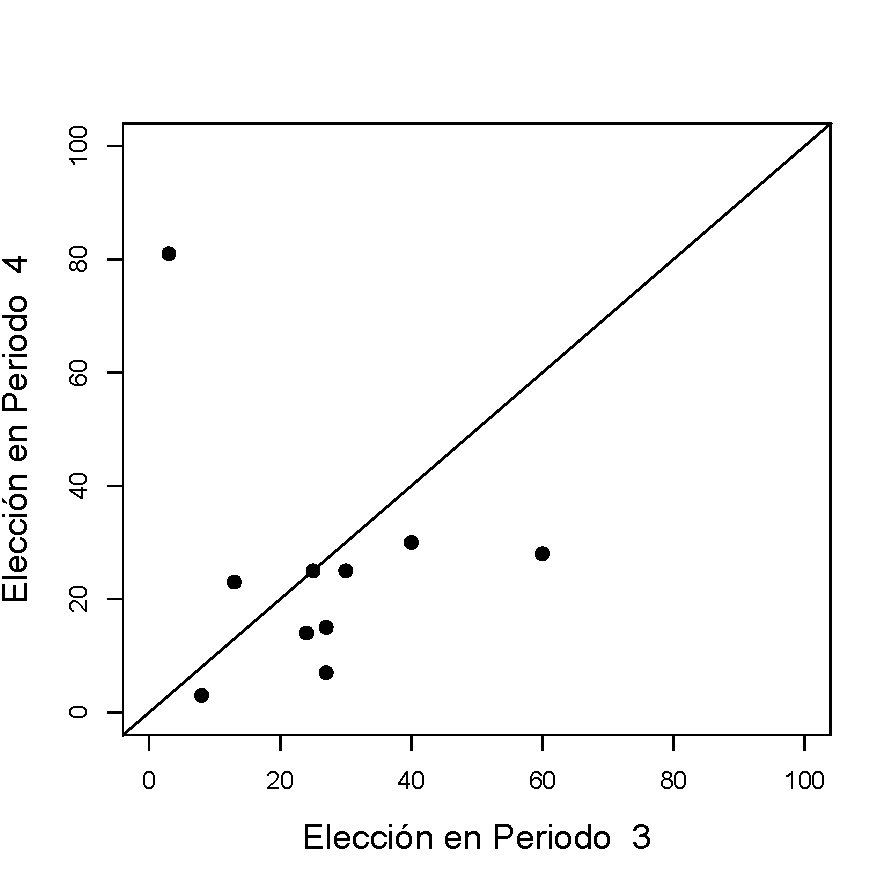
\includegraphics[width=0.45\textwidth]{Figures/F6_3} & 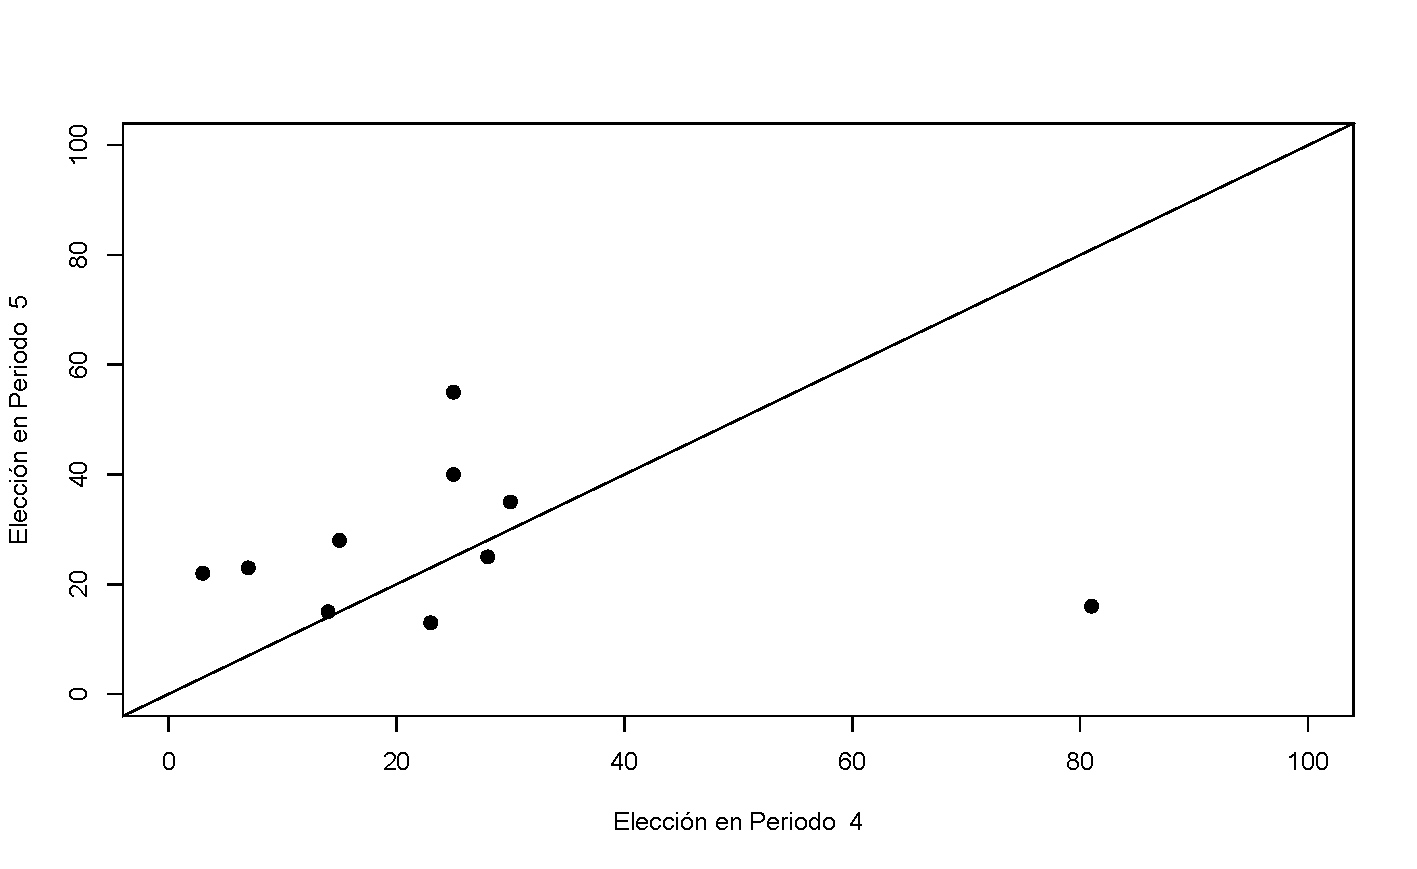
\includegraphics[width=0.45\textwidth]{Figures/F6_4} 
\decoRule
\caption[Elecciones registradas en ensayos consecutivos]{Se presenta la relación entre los números elegidos en periodos consecutivos por los participantes A, quienes no sólo jugaron los cuatro periodos del Subjuego 1, sino que permanecieron a lo largo del Subjuego 2. En los primeros tres páneles se aprecia que en el Subjuego 1 las elecciones tendían a disminuir, mientras que en el último panel, se observa un incremento en las mismas (el Efecto Reset).}
\label{fig:Reset_cambios}
\end{figure}

Se realizó una prueba Binomial bayesiana de una cola para comparar contra el azar la proporción de participantes A que aumentaban o disminuían sus elecciones entre cada uno de los primeros cinco periodos que jugaron (ver Tabla~\ref{Binom_Reset}), encontrando evidencia anecdótica. La falta de robustez en los resultados obtenidos en esta prueba puede deberse a que sólamente se realizaron 10 sesiones experimentales.\\

\begin{table}[h]
\caption[Prueba binomial bayesiana para evaluar la proporción de casos en que los participantes A aumentan y reducen su número elegido]{\textbf{Cambios en los números elegidos en periodos consecutivos} Prueba binomial bayesiana que compara contra el azar el número de veces que el número elegido en periodos consecutivos aumentaba o disminuía.}
\label{Binom_Reset}
\centering
\begin{tabular}{l c | c c | c}
\toprule
%\tabhead{Groups} & \tabhead{Treatment X} & \tabhead{Treatment Y} \\
\textbf{Periodos} & \textbf{Cambio} & \textbf{Casos} & \textbf{Proporción} & \textbf{$BF_{10}$}\\
\midrule
1 vs 2 & aumentó & 3 & 0.3 & 0.176\\
       & disminuyó & 7 & 0.7 & 1.376\\
2 vs 3 & aumentó & 4 & 0.4 & 0.243\\
       & disminuyó & 6 & 0.6 & 0.643\\
3 vs 4 & aumentó & 2 & 0.2 & 0.135\\
       & disminuyó & 8 & 0.8 & 4.002\\
5 vs 6 & aumentó & 7 & 0.7 & 1.376\\
       & disminuyó & 3 & 0.3 & 0.176\\
\bottomrule
\end{tabular}
\end{table}

Para determinar si, en promedio, el número elegido por el participante A en el último periodo del Subjuego 1 es menor que el número elegido en el primer periodo del Subjuego 2, se realizó una prueba t de una cola, donde se encontró que si bien el promedio de los números elegidos en el primer periodo del Subjuego 2 es mayor que el promedio de las elecciones regitradas al final del Subjuego 1, la diferencia parece ser pequeña y no significativa.\\

No obstante, al revisar los datos de cada sesión experimental se encontraron anomalías en la ejecución del participante A de la Sesión 3, cuyo comportamiento difiere considerablemente de lo que se reporta en la literatura y en el resto de las sesiones realizadas en la presente investigación.\\

En la Figura~\ref{fig:Elecciones_ParticipantesA} se presentan las elecciones de los participantes para cada uno de los ocho periodos jugados en los dos Subjuegos, en cada una de las diez sesiones experimentales. Se puede apreciar que el participante A de la Sesión 3 no presenta la tendencia a elegir números más pequeños periodo a periodo y por el contrario, elige números muy grandes en el último periodo de cada subjuego, una estrategia que no aporta ningún tipo de ventaja en el juego. Este patrón de respuesta sugiere que el participante A de la Sesión 3 pudo no haber entendido la dinámica del juego.\\

\begin{figure}[hp]
\centering
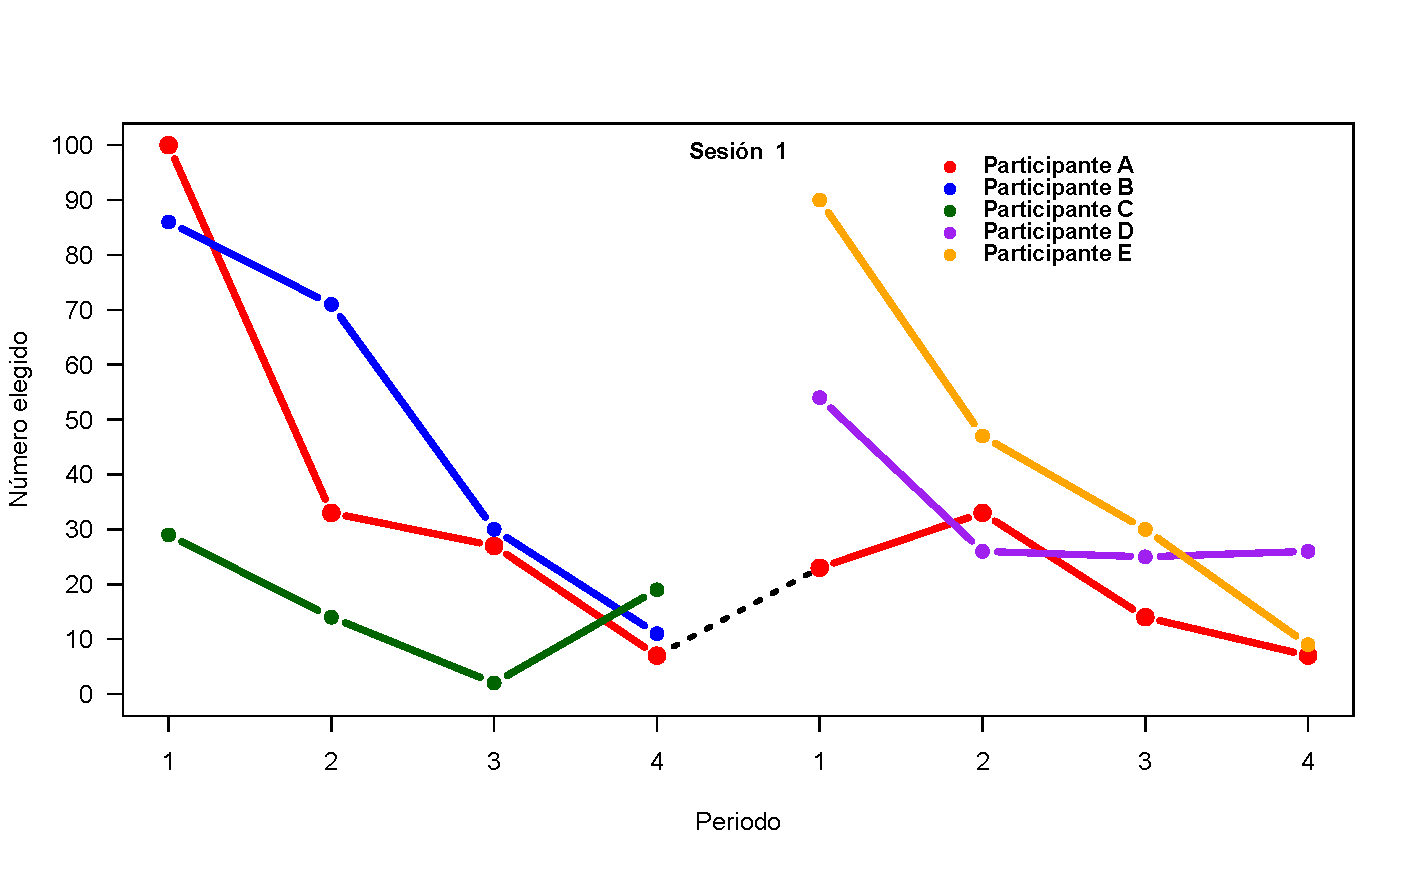
\includegraphics[width=0.45\textwidth]{Figures/F7_1} & 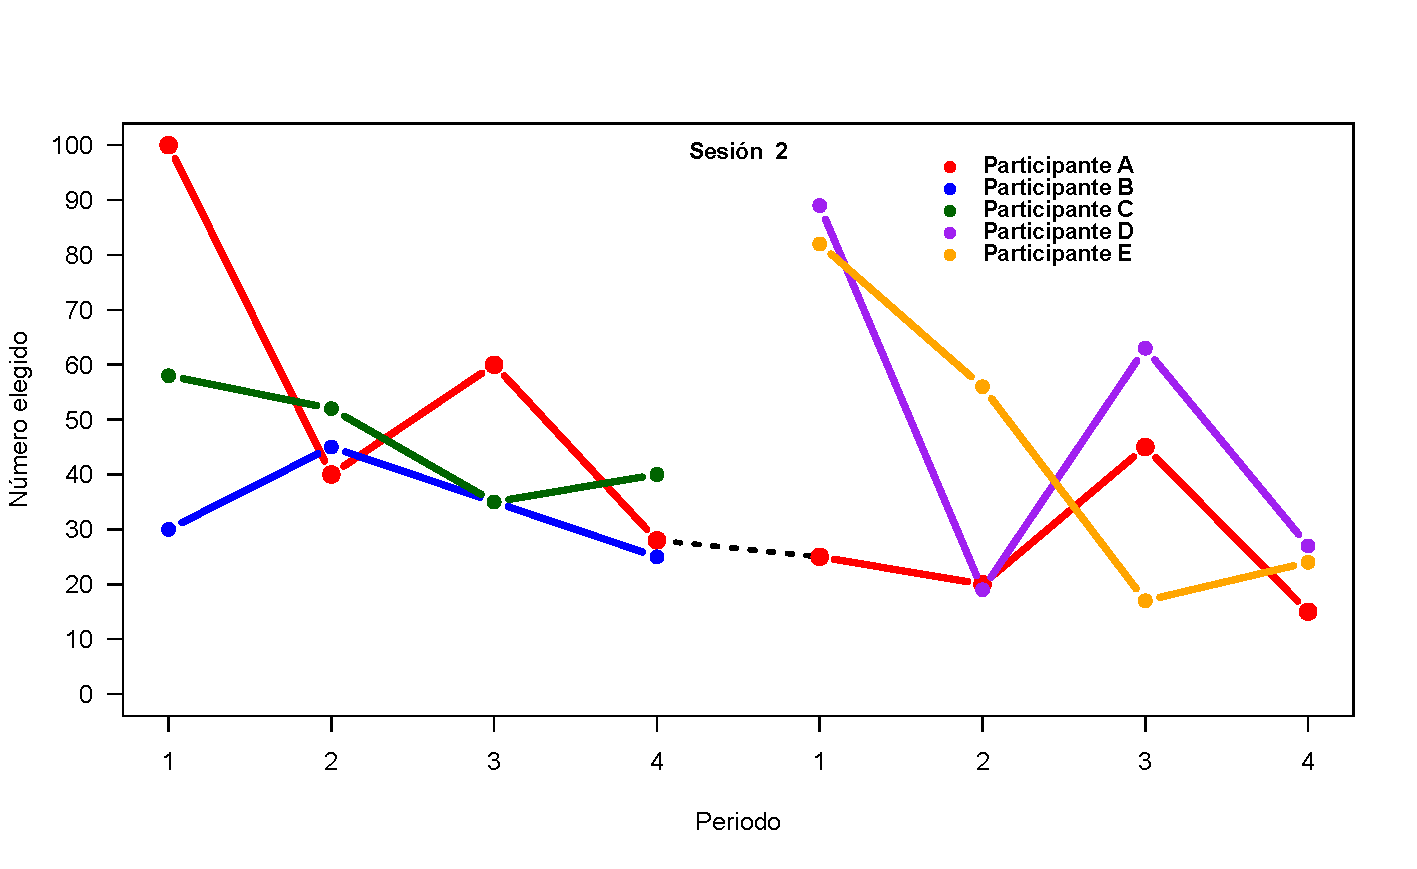
\includegraphics[width=0.45\textwidth]{Figures/F7_2} 
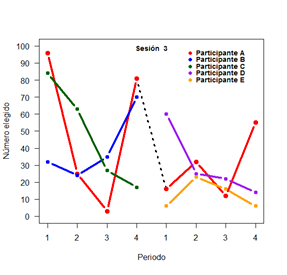
\includegraphics[width=0.45\textwidth]{Figures/F7_3} & 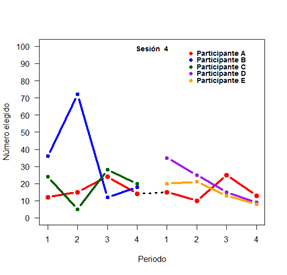
\includegraphics[width=0.45\textwidth]{Figures/F7_4} 
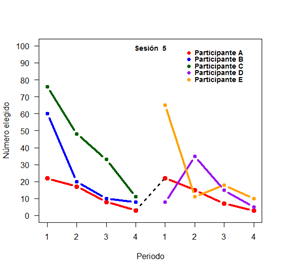
\includegraphics[width=0.45\textwidth]{Figures/F7_5} & 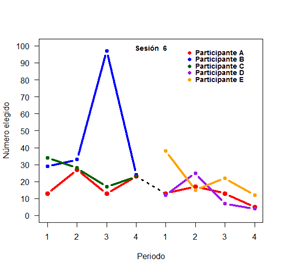
\includegraphics[width=0.45\textwidth]{Figures/F7_6} 
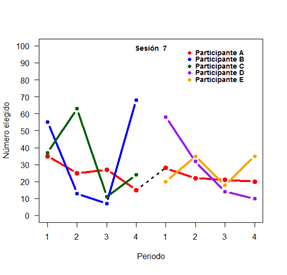
\includegraphics[width=0.45\textwidth]{Figures/F7_7} & 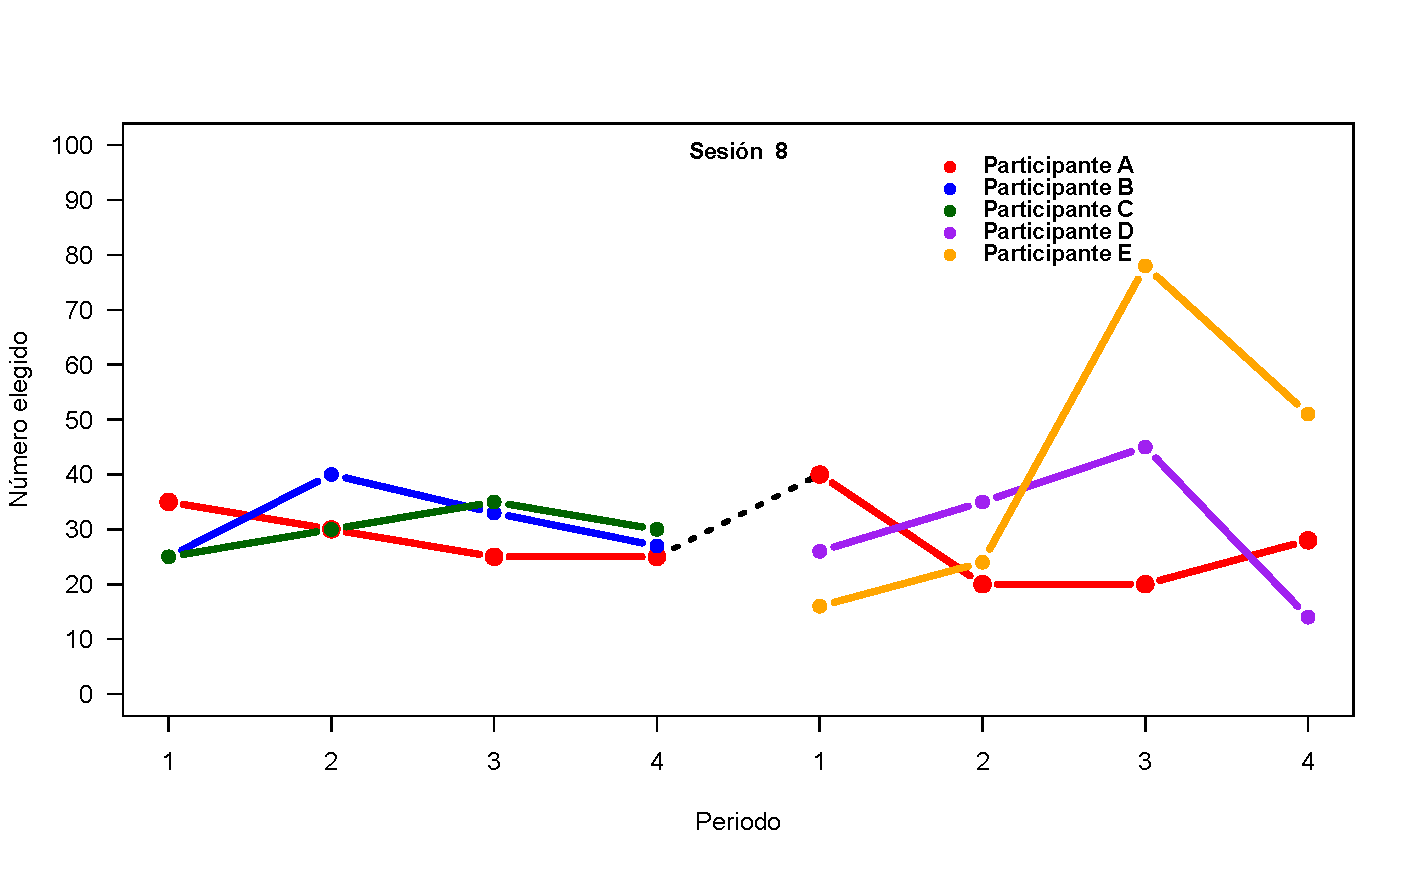
\includegraphics[width=0.45\textwidth]{Figures/F7_8} 
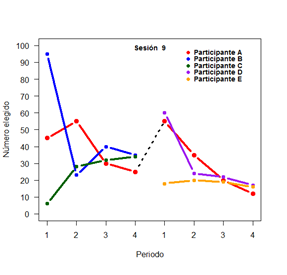
\includegraphics[width=0.45\textwidth]{Figures/F7_9} & 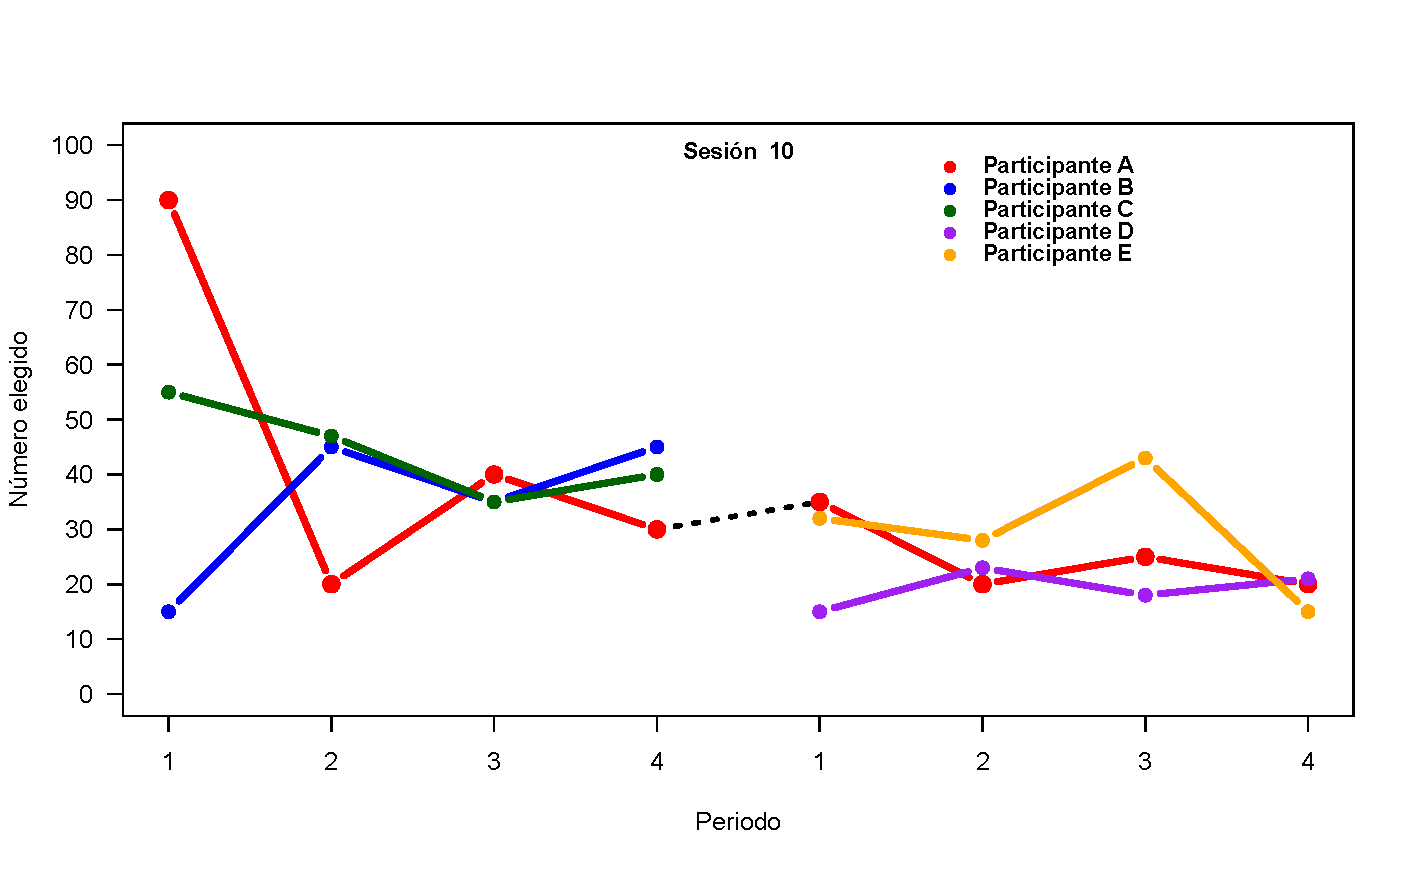
\includegraphics[width=0.45\textwidth]{Figures/F7_10} 
\decoRule
\caption[Elecciones de todos los participantes]{Se presentan las elecciones de los participantes en las diez sesiones experimentales raelizadas, en los Subjuegos 1 y 2. Se puede apreciar que el participante A de la sesión 3 tiene un patrón atípico respecto del resto de las sesiones y de lo que se esperaría de acuerdo a la literatura.}
\label{fig:Elecciones_ParticipantesA}
\end{figure}  
  
Para evaluar qué tan saliente es la tirada del participante A de la sesión 3 en el primer periodo del Subjuego 2, en la Figura~\ref{fig:Boxplot} se presentan dos diagramas: El primero, de caja y bigotes, muestra que la elección realizada por el jugador A de la Sesión 3 en el primer periodo se encuentra por arriba del rango intercuadrático multiplicado por 1.5, lo que permite clasificarla como un valor atípico.  El  segundo diagrama, de violín, complementa la información del diagrama de caja y bigotes con un diagrama de densidad a los lados; la forma externa del diagrama representa todos los resultados posibles, y el grosor indica qué tan comúnes son.\\

\begin{figure}[hp]
\centering
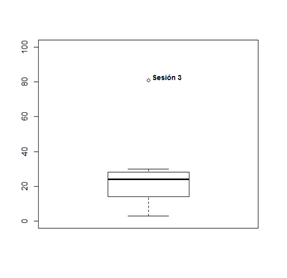
\includegraphics[width=0.45\textwidth]{Figures/F8_1} & 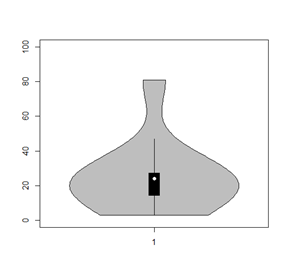
\includegraphics[width=0.45\textwidth]{Figures/F8_2} 
\decoRule
\caption[Participante atípico: Comparando el desempeño del Participante A de la Sesión 3]{Comparación del desempeño de los participantes A con el desempeño observado en la Sesión 3. Del lado izquiero e presenta un diagrama de caja y bigotes, donde se puede apreciar que el desempeño registrado en la Sesión 3 está muy alejado del resto. Del lado derecho, un diagrama de violín, que complementa esta información con un diagrama de densidad.}
\label{fig:Boxplot}
\end{figure}  

Tomando en cuenta dicho resultado, se repitieron las pruebas t de una cola para comprobar que el número elegido por los participantes A en el último periodo del Subjuego 1 son más pequeños que el número elegido en el primer periodo del Subjuego 2, omitiendo al participante A de la Sesión 3. Al realizar dicho análisis, el número elegido en promedio por los participantes A en el último periodo del subjuego 1 fue significativamente menor que la elección promedio registrada en el primer periodo del subjuego 2, encontrando evidencia del efecto de reset (prueba clásica $t = -2.317$, $p = .025 < 0.5$, prueba bayesiana $BF_10 = 3.57$, $error = 1.377e-4$).\\

En la Figura~\ref{fig:ParticipantesA_promedio} se presenta el promedio de los números elegidos por los participantes A y los participantes no-A (participantes B y C, D y E para los Subjuegos 1 y 2, respectivamente) en cada periodo. Se presentan en gráficos diferentes los promedios computados cuando se consideran los datos de la Sesión 3 (panel izquierdo) y cuando no (panel derecho).\\
  
\begin{figure}[h]
\centering
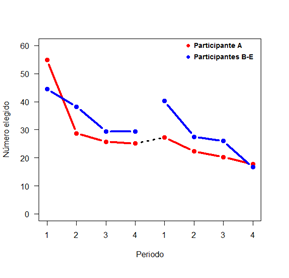
\includegraphics[width=0.45\textwidth]{Figures/F9_1} & 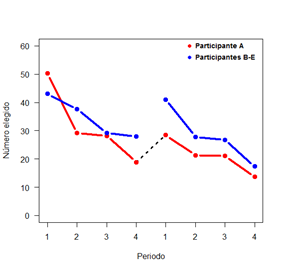
\includegraphics[width=0.45\textwidth]{Figures/F9_2} 
\decoRule
\caption[Promedio de los números elegidos por los participantes A y no-A en cada uno de los periodos jugados]{Se presenta el promedio de los números elegidos en cada uno de los periodos jugados por los participantes A (en color rojo) y los participantes B y C en el Subjuego 1 y los participantes D y E en el Subjuego 2 (en color azul). La gráfica de la izquierda incorpora los datos obtenidos en la Sesión 3 y la gráfica de la derecha, no.}
\label{fig:ParticipantesA_promedio}
\end{figure}  

Con base en estos resultados, se puede afirmar que se logró replicar el efecto de reset reportado por Slonim (\citeyear{Slonim}), omitiendo los datos recopilados de la Sesión 3. Con ello, se comprueba la validez en la comparación de la consistencia entre las creencias y elecciones de los participantes A en cada periodo, a lo largo de los dos subjuegos.\\

\section{Consistencia entre creencias y elecciones entre subjuegos}\\

Las creencias y elecciones de los participantes en el Subjuego 2 fueron sometidos a los mismos análisis reportados para el subjuego 1 en la \textbf{sección 4.2}: se computaron las Diferencias Normalizadas y las Diferencias Relativas, incluyendo y excluyendo la multiplicación por $p$. Pero en esta ocasión, se hizo una distinción entre la ejecución de los jugadores con experiencia (participantes A) y los jugadores que participaban en el juego por primera vez (participantes D y E).\\

En la figura~\ref{fig:Consistencia_promedio} se contrasta la elección de cada participante con su creencia promedio para cada uno de los periodos del subjuego 2, cuando se incluye la multiplicación por $p$ y cuando esta se omite. Los participantes A están marcados en rojo. En general, se observa que estos participantes fueron más consistentes en sus creencias y elecciones comparados con los participantes D y E.\\

\begin{figure}[hp]
\centering
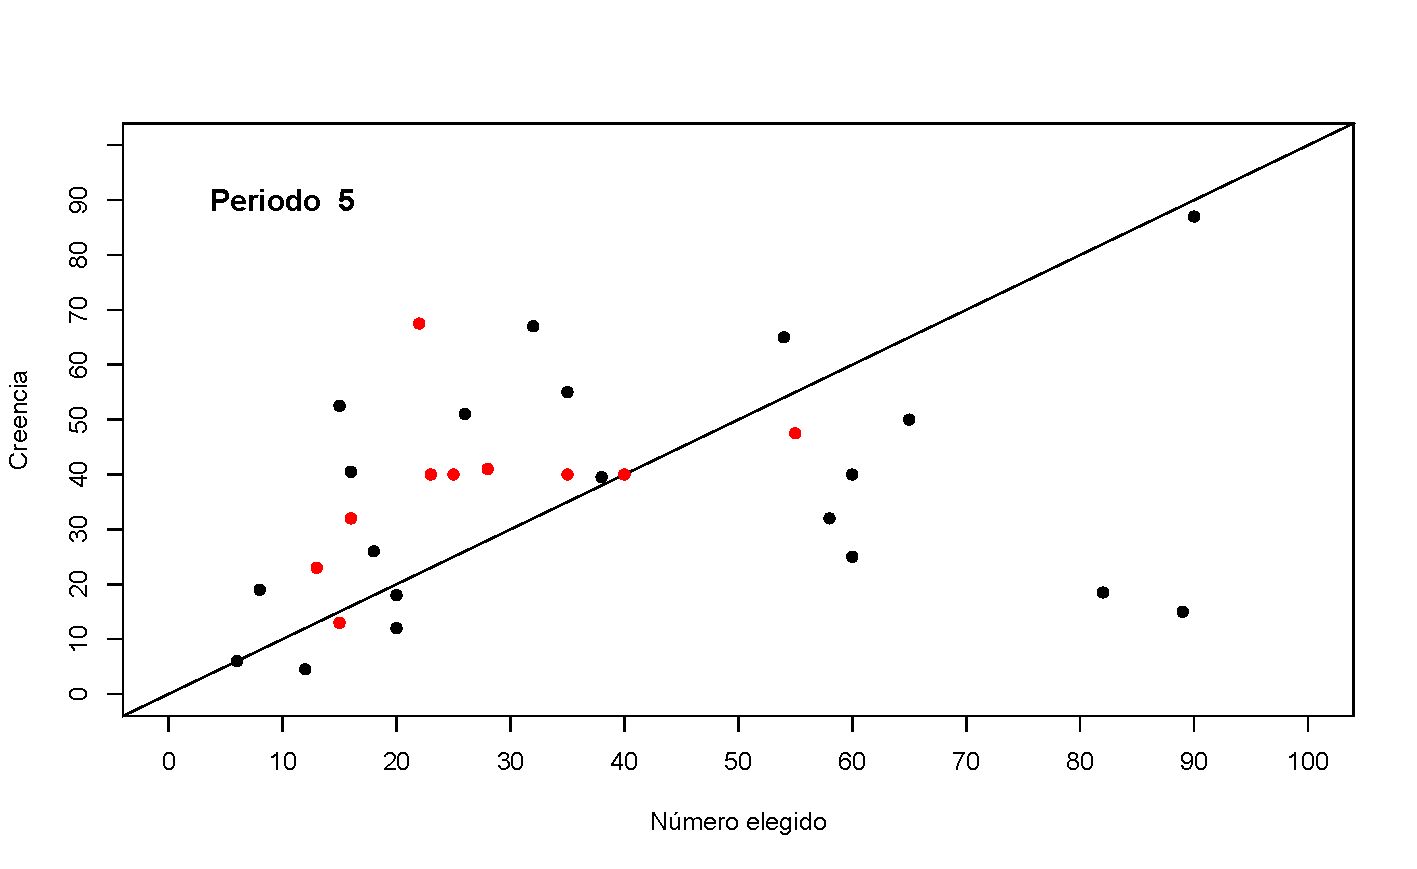
\includegraphics[width=0.45\textwidth]{Figures/F10_1} & 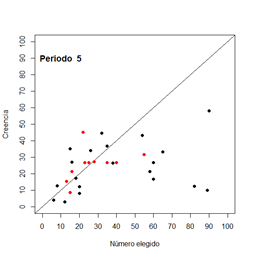
\includegraphics[width=0.45\textwidth]{Figures/F10_2} 
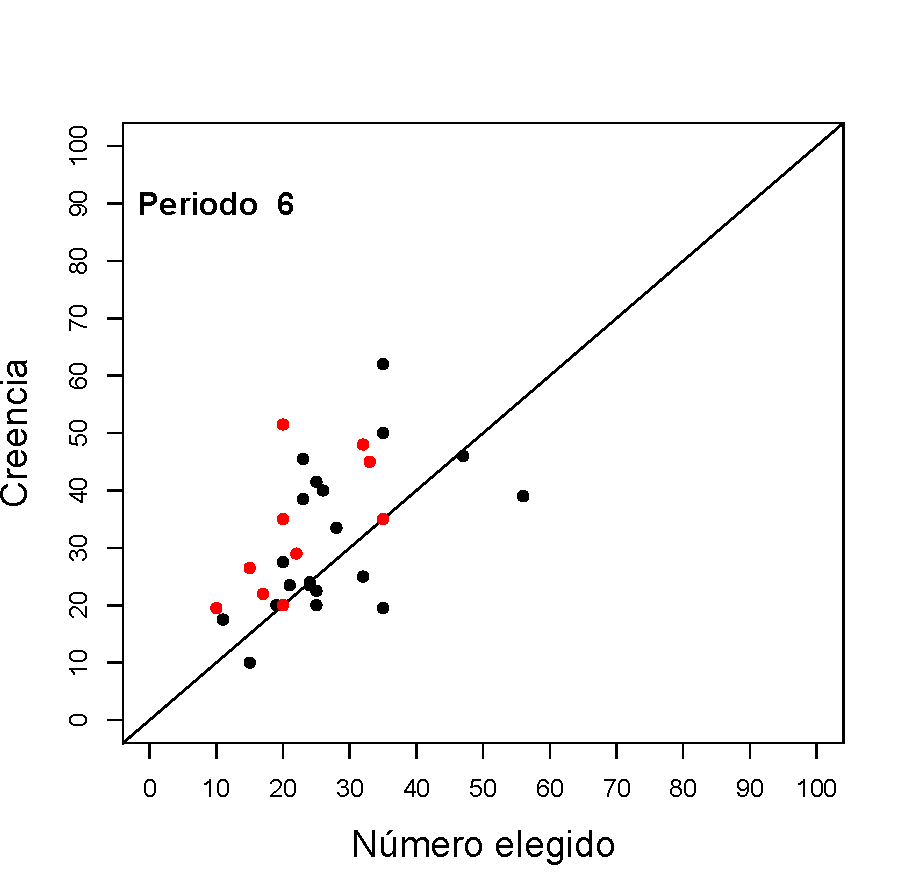
\includegraphics[width=0.45\textwidth]{Figures/F10_3} & 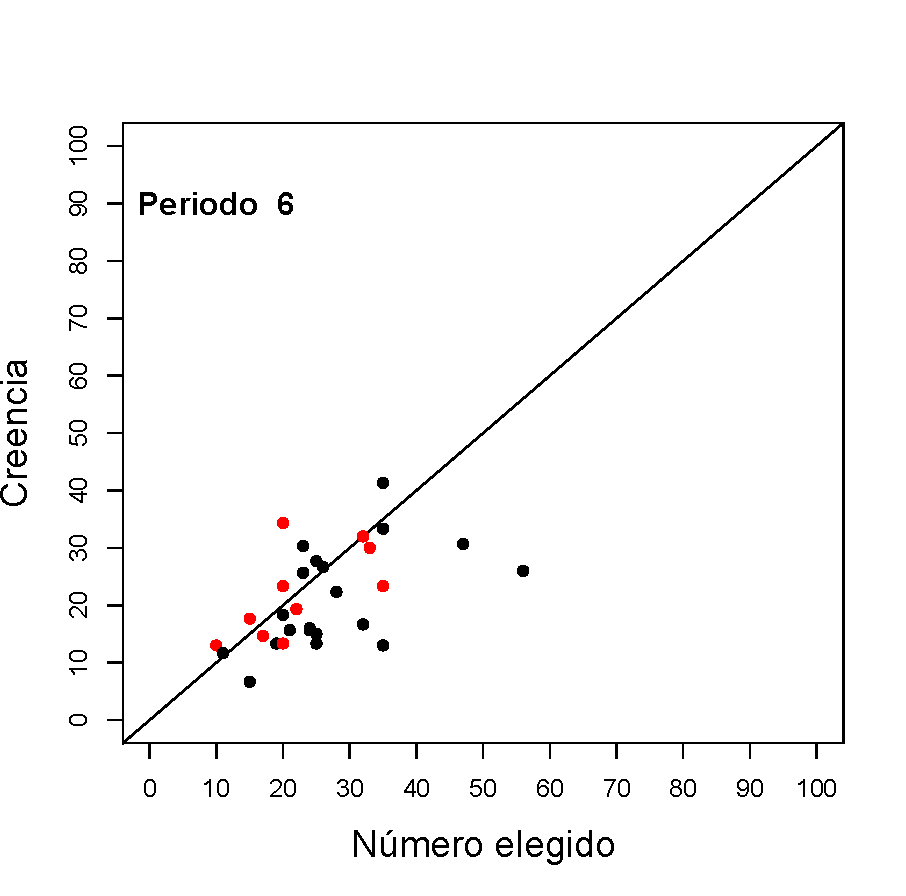
\includegraphics[width=0.45\textwidth]{Figures/F10_4} 
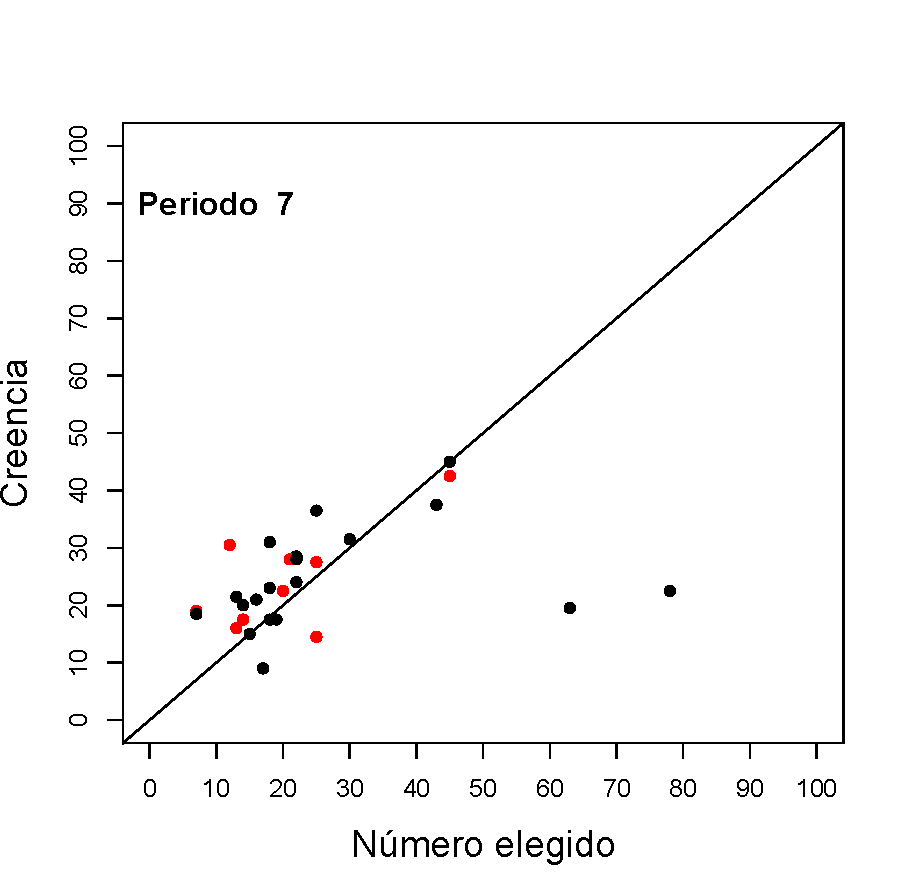
\includegraphics[width=0.45\textwidth]{Figures/F10_5} & 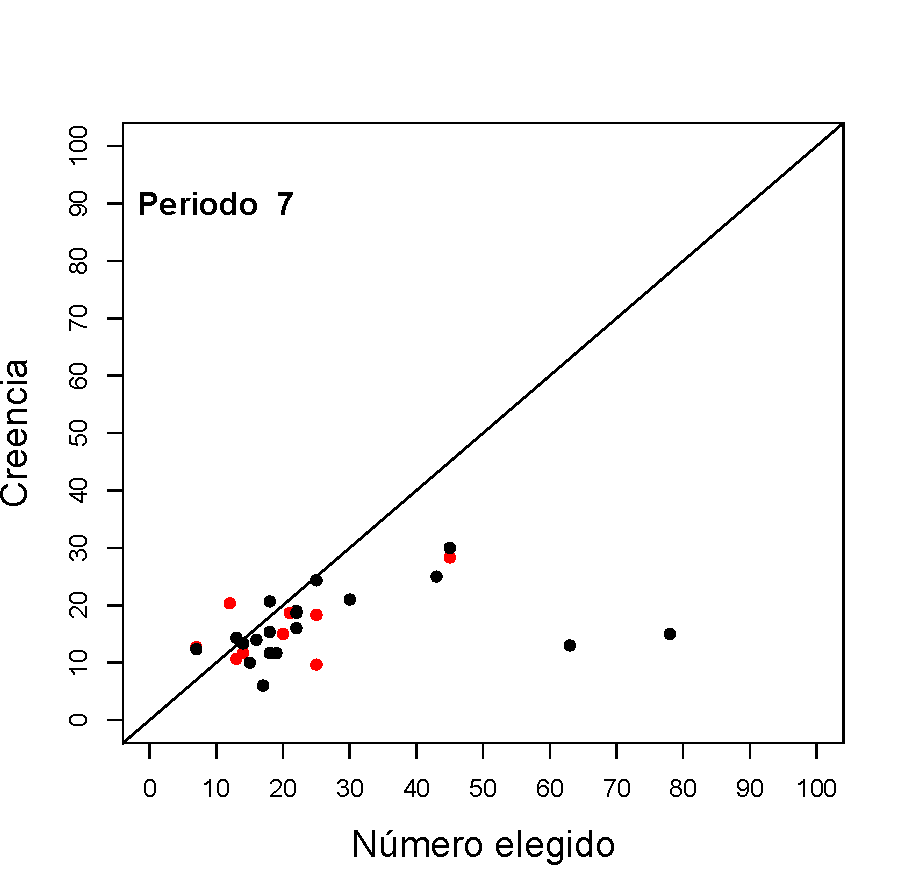
\includegraphics[width=0.45\textwidth]{Figures/F10_6} 
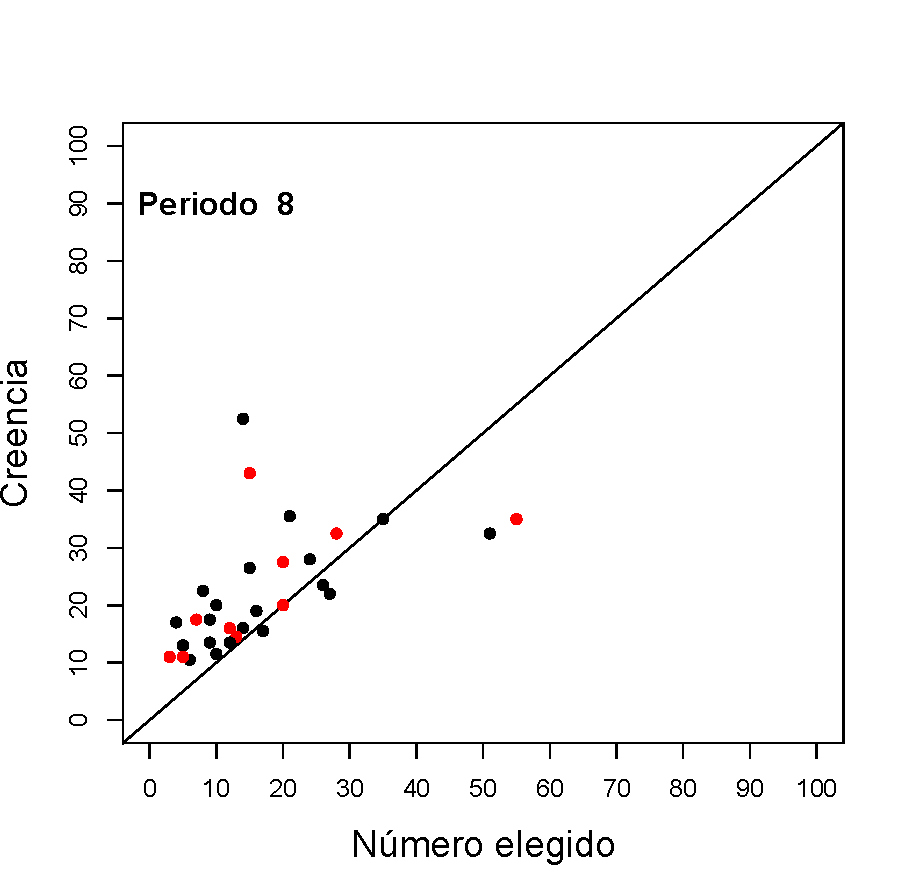
\includegraphics[width=0.45\textwidth]{Figures/F10_7} & 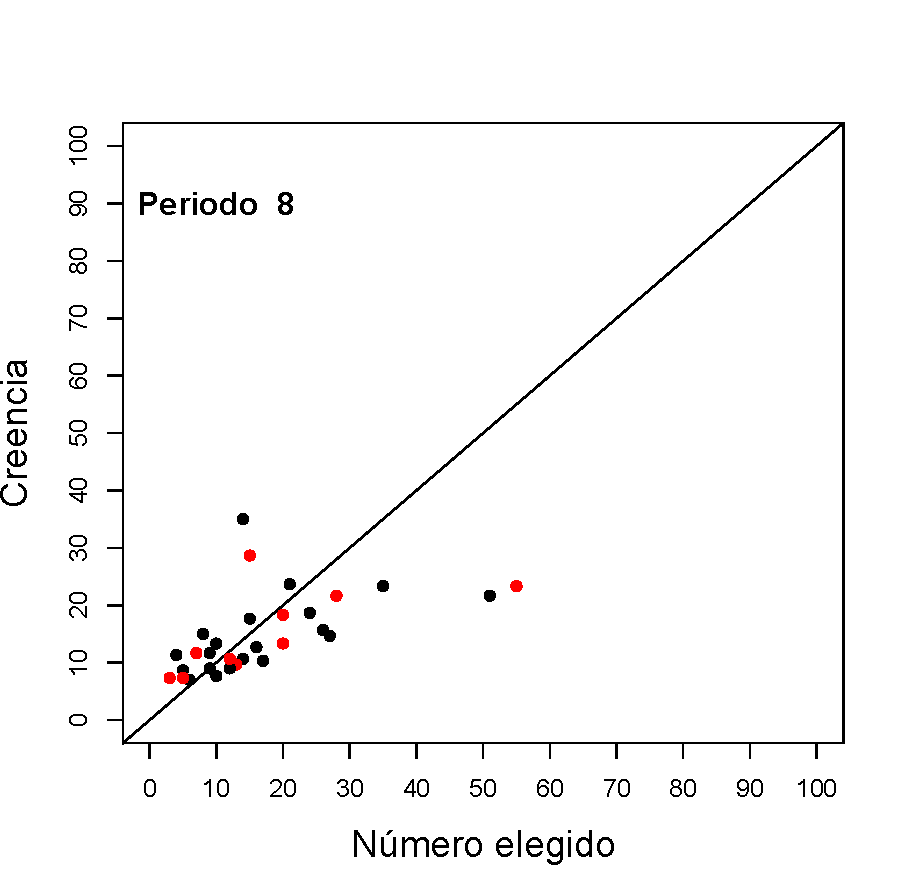
\includegraphics[width=0.45\textwidth]{Figures/F10_8} 
\decoRule
\caption[Comparación enter las creencias y elecciones registradas en el Subjuego 2]{Se presenta la relación entre el promedio de las creencias registradas en cada periodo por los participantes del Subjuego 2 y sus elecciones, cuando sus creencias son multiplicadas por $p$ (paneles izquierdos) o no (páneles derechos). Los participantes A, que ya tenían la experiencia de haber jugado en el Subjuego 1, se señalan en rojo.}
\label{fig:Consistencia_promedio}
\end{figure}  

Se calculó la Diferencia Normalizada entre las creencias y elecciones registradas en cada periodo del Subjuego 2, por los participantes A y los participantes D y E. Posteriormente,  se realizaron pruebas t bayesianas para determinar si estas diferencias fueron estadísticamente diferentes de 0.\\

En las Tablas~\ref{DN-S2-A-B} y \ref{DN-S2-DyE-B} se presentan los resultados obtenidos en las pruebas t bayesianas de una sola muestra que evalúan el promedio de las Diferencias Normalizadas computadas entre creencias y elecciones contra 0. De acuerdo con la Tabla~\ref{DN-S2-A-B}, los participantes A no mostraron diferencias significativas (el factor de Bayes en este caso indica qué tantas veces es más que no haya diferencias), lo que indica una mayor consistencia entre sus creencias y elecciones en todos los periodos del subjuego 2. En contraste, en la Tabla~\ref{DN-S2-DyE-B} se puede observar que los participantes D y E mostraron diferencias significativas en los primeros tres periodos del subjuego, y sólo parecieron  adquirir consistencia entre sus creencias y elecciones en el último periodo. Este último resultado es muy similar a lo reportado en los participantes del Subjuego 1, donde todos los jugadores compartían el mismo nivel de experiencia. Además, en todos los casos, las creencias estuvieron por debajo de las elecciones reales. En las Figuras~\ref{fig:DN_S2_A} y \ref{fig:DN_S2_DyE} se incluyen las distribuciones prior y posterior de las Diferencias Normalizadas por periodo para los participantes A y los participantes D y E, respectivamente.\\ 

\begin{table}[h]
\caption[Diferencias Normalizadas en el Subjuego 2; Participante A (Pruebas t de una muestra)]{\textbf{Diferencias Normalizadas en el Subjuego 2 (Participantes A)} Se presentan los resultados de una prueba t de una muestra que compara contra 0 las Diferencias Normalizadas computadas para los participantes A en el Subjuego 2}
\label{DN-S2-A-B}
\centering
\begin{tabular}{l | c c | c}
\toprule
%\tabhead{Groups} & \tabhead{Treatment X} & \tabhead{Treatment Y} \\
\textbf{} & \textbf{$BF_{01}$} & \textbf{$error\%$} & \textbf{Diferencia promedio}\\
\midrule
Periodo 5 & 3.010 & 0.006 & -0.049\\
Periodo 6 & 3.212 & 0.007 & -0.011\\
Periodo 7 & 2.012 & 0.003 & -0.133\\
Periodo 8 & 3.205 & 0.007 & -0.028\\
\bottomrule
\end{tabular}
\end{table}

\begin{table}[h]
\caption[Diferencias Normalizadas en el Subjuego 2; Participante A (Pruebas t de una muestra)]{\textbf{Diferencias Normalizadas en el Subjuego 2 (Participantes A)} Se presentan los resultados de una prueba t de una muestra que compara contra 0 las Diferencias Normalizadas computadas para los participantes A en el Subjuego 2}
\label{DN-S2-DyE-B}
\centering
\begin{tabular}{l | c c | c}
\toprule
%\tabhead{Groups} & \tabhead{Treatment X} & \tabhead{Treatment Y} \\
\textbf{} & \textbf{$BF_{01}$} & \textbf{$error\%$} & \textbf{Diferencia promedio}\\
\midrule
Periodo 5 & 0.315 & 0.003 & -0.349\\
Periodo 6 & 0.102 & 6.001e-4 & -0.243\\
Periodo 7 & 0.063 & 2.519e^-4 & -0.307\\
Periodo 8 & 4.002 & 0.022 & -0.047\\
\bottomrule
\end{tabular}
\end{table}
  

\begin{figure}[hp]
\centering
\includegraphics[width=0.45\textwidth]{Figures/F11_1} & \includegraphics[width=0.45\textwidth]{Figures/F11_2} 
\includegraphics[width=0.45\textwidth]{Figures/F11_3} & \includegraphics[width=0.45\textwidth]{Figures/F11_4} 
\decoRule
\caption[Evaluación de las Diferencias Normalizadas entre creencias y elecciones en los participantes A en el Subjuego 2 (Factor de Bayes)]{Como resultado de la evaluación de las Diferencias Normalizadas computadas entre las creencias y las elecciones de los participantes A en el Subjuego 2, se presenta la comparación entre las densidades de probabilidad de las distribuciones prior (hipótesis nula) y posterior (hipótesis alterna) computadas por cada periodo, en el punto de no diferencia ($\delta = 0$).}
\label{fig:DN_S2_A}
\end{figure}  


\begin{figure}[hp]
\centering
\includegraphics[width=0.45\textwidth]{Figures/F12_1} & \includegraphics[width=0.45\textwidth]{Figures/F12_2} 
\includegraphics[width=0.45\textwidth]{Figures/F12_3} & \includegraphics[width=0.45\textwidth]{Figures/F12_4} 
\decoRule
\caption[Evaluación de las Diferencias Normalizadas entre creencias y elecciones en los participantes D y E en el Subjuego 2 (Factor de Bayes)]{Como resultado de la evaluación de las Diferencias Normalizadas computadas entre las creencias y las elecciones de los participantes D y E en el Subjuego 2, se presenta la comparación entre las densidades de probabilidad de las distribuciones prior (hipótesis nula) y posterior (hipótesis alterna) computadas por cada periodo, en el punto de no diferencia ($\delta = 0$).}
\label{fig:DN_S2_DyE}
\end{figure}  

Se repitió el cálculo de las Diferencias Normalizadas en los cuatro periodos del Subjuego 2 omitiendo la multiplicación por $p$, con el propósito de evaluar si los jugadores tomaron en cuenta este cálculo en la elección de su número. Tras la realización de las pruebas t bayesianas de una sola muestra correspondientes,  sólo se encontraron diferencias significativas entre las elecciones y las creencias de los participantes A en los dos primeros  periodos, (ver Tabla~\ref{DNnop-S2-A-B}). En general, la magnitud de las diferencias parece ser mayor en todos los periodos cuando se excluye la multiplicación por $p$ que cuando esta sí se incluye. Este resultado sugiere que los jugadores con experiencia previa sí tomaron en cuenta la multiplicación por $p$, o por lo menos, que aprendieron desde el Subjuego 1 que el número objetivo siempre está por debajo del promedio de los números elegidos.\\

Por otra parte, en el caso de los participantes sin experiencia (D y E) solo se encontraron diferencias significativas respecto de 0 en el último periodo (ver Tabla~\ref{DNnop-S2-DyE-B}), resultado que coincide con lo reportado en el Subjuego 1, sugiriendo nuevamente que los participantes incorporaron la multiplicación por $p$ (o comprendieron la tendencia del juego hacia el equilibrio)  sólo después de varias repeticiones. Así mismo, en las Figuras~\ref{fig:DNnop_S2_A} y \ref{fig:DNnop_S2_DyE} se presentan las distribuciones prior y posterior computadas con las pruebas t realizadas por cada periodo, para los participantes con y sin experiencia, respectivamente.\\

\begin{table}[h]
\caption[Diferencias Normalizadas en el Subjuego 2 omitiendo la multiplicación por $p$; Participante A (Pruebas t de una muestra)]{\textbf{Diferencias Normalizadas en el Subjuego 2 (Participantes A)} Se presentan los resultados de una prueba t de una muestra que compara contra 0 las Diferencias Normalizadas computadas para los participantes A en el Subjuego 2, cuando las creencias registradas no son multiplicadas por $p$.}
\label{DNnop-S2-A-B}
\centering
\begin{tabular}{l | c c | c}
\toprule
%\tabhead{Groups} & \tabhead{Treatment X} & \tabhead{Treatment Y} \\
\textbf{} & \textbf{$BF_{01}$} & \textbf{$error\%$} & \textbf{Diferencia promedio}\\
\midrule
Periodo 5 & 0.537 & 0.001 & 0.333\\
Periodo 6 & 0.046 & 9.917e-5 & 0.414\\
Periodo 7 & 1.274 & 0.004 & 0.238\\
Periodo 8 & 0.643 & 0.003 & 0.438\\
\bottomrule
\end{tabular}
\end{table}


\begin{table}[h]
\caption[Diferencias Normalizadas en el Subjuego 2, omitiendo la multiplicación por $p$; Participantes D y E (Pruebas t de una muestra)]{\textbf{Diferencias Normalizadas en el Subjuego 2 (Participantes D y E)} Se presentan los resultados de una prueba t de una muestra que compara contra 0 las Diferencias Normalizadas computadas para los participantes D y E en el Subjuego 2, cuando las creencias registradas no se multiplican por $p$.}
\label{DNnop-S2-DyE-B}
\centering
\begin{tabular}{l | c c | c}
\toprule
%\tabhead{Groups} & \tabhead{Treatment X} & \tabhead{Treatment Y} \\
\textbf{} & \textbf{$BF_{01}$} & \textbf{$error\%$} & \textbf{Diferencia promedio}\\
\midrule
Periodo 5 & 4.265 & 0.022 & 0.024\\
Periodo 6 & 1.417 & 0.004 & 0.170\\
Periodo 7 & 3.541 & 0.021 & 0.071\\
Periodo 8 & 0.115 & 7.221e^-4 & 0.440\\
\bottomrule
\end{tabular}
\end{table}
  

\begin{figure}[hp]
\centering
\includegraphics[width=0.45\textwidth]{Figures/F13_1} & \includegraphics[width=0.45\textwidth]{Figures/F13_2} 
\includegraphics[width=0.45\textwidth]{Figures/F13_3} & \includegraphics[width=0.45\textwidth]{Figures/F13_4} 
\decoRule
\caption[Evaluación de las Diferencias Normalizadas entre creencias (sin multiplicar por $p$) y elecciones en los participantes A en el Subjuego 2 (Factor de Bayes)]{Como resultado de la evaluación de las Diferencias Normalizadas computadas entre las creencias (omitiendo la multiplicación por $p$) y las elecciones de los participantes A en el Subjuego 2, se presenta la comparación entre las densidades de probabilidad de las distribuciones prior (hipótesis nula) y posterior (hipótesis alterna) computadas por cada periodo, en el punto de no diferencia ($\delta = 0$).}
\label{fig:DNnop_S2_A}
\end{figure}  


\begin{figure}[hp]
\centering
\includegraphics[width=0.45\textwidth]{Figures/F14_1} & \includegraphics[width=0.45\textwidth]{Figures/F14_2} 
\includegraphics[width=0.45\textwidth]{Figures/F14_3} & \includegraphics[width=0.45\textwidth]{Figures/F14_4} 
\decoRule
\caption[Evaluación de las Diferencias Normalizadas entre creencias y elecciones en los participantes D y E en el Subjuego 2 (Factor de Bayes)]{Como resultado de la evaluación de las Diferencias Normalizadas computadas entre las creencias no multiplicadas por $p$ y las elecciones de los participantes D y E en el Subjuego 2, se presenta la comparación entre las densidades de probabilidad de las distribuciones prior (hipótesis nula) y posterior (hipótesis alterna) computadas por cada periodo, en el punto de no diferencia ($\delta = 0$).}
\label{fig:DNnop_S2_DyE}
\end{figure}  

Posteriormente, se computaron las Diferencias Relativas entre las creencias y elecciones registradas en los cuatro periodos del Subjuego 2 y se realizaron pruebas t bayesianas para determinar si estas eran significativamente diferentes de 0. Los resultados de este análisis se presentan en la Tabla~\ref{DR-S2-A-B} para el participante A y en la Tabla~\ref{DR-S2-DyE-B} para los participantes D y E.\\

\begin{table}[h]
\caption[Diferencias Relativas en el Subjuego 2; Participantes A (Pruebas t de una muestra)]{\textbf{Diferencias Relativas en el Subjuego 2 (Participantes A)} Se presentan los resultados de una prueba t de una muestra que compara contra 0 las Diferencias Normalizadas computadas para los participantes D y E en el Subjuego 2.}
\label{DR-S2-A-B}
\centering
\begin{tabular}{l | c c | c}
\toprule
%\tabhead{Groups} & \tabhead{Treatment X} & \tabhead{Treatment Y} \\
\textbf{} & \textbf{$BF_{01}$} & \textbf{$error\%$} & \textbf{Diferencia promedio}\\
\midrule
Periodo 5 & 3.085 & 0.006 & -0.042\\
Periodo 6 & 3.231 & 0.007 & -0.007\\
Periodo 7 & 1.831 & 0.002 & -0.162\\
Periodo 8 & 3.165 & 0.007 & 0.038\\
\bottomrule
\end{tabular}
\end{table}

\begin{table}[h]
\caption[Diferencias Relativas en el Subjuego 2; Participantes D y E (Pruebas t de una muestra)]{\textbf{Diferencias Normalizadas en el Subjuego 2 (Participantes D y E)} Se presentan los resultados de una prueba t de una muestra que compara contra 0 las Diferencias Relativas computadas para los participantes D y E en el Subjuego 2.}
\label{DR-S2-DyE-B}
\centering
\begin{tabular}{l | c c | c}
\toprule
%\tabhead{Groups} & \tabhead{Treatment X} & \tabhead{Treatment Y} \\
\textbf{} & \textbf{$BF_{01}$} & \textbf{$error\%$} & \textbf{Diferencia promedio}\\
\midrule
Periodo 5 & 0.272 & 0.002 & -0.407\\
Periodo 6 & 0.044 & 3.044e^-4 & -0.283\\
Periodo 7 & 0.080 & 4.394e^-4 & -0.341\\
Periodo 8 & 4.295 & 0.022 & -0.007\\
\bottomrule
\end{tabular}
\end{table}
  
 Los resultados que se obtienen son muy similares a lo que se observa al utilizar el método de Diferencias Normalizadas: el participante A muestra ser consistente en los cuatro periodos y los participantes D y E son inconsistencias en los primeros tres. En las Figuras~\ref{fig:DR_S2_A} y \ref{fig:DR_S2_DyE} se incluyen las distribuciones prior y posterior computadas como resultado de las pruebas t bayesianas realizadas por periodo, por cada tipo de participante.\\

\begin{figure}[hp]
\centering
\includegraphics[width=0.45\textwidth]{Figures/F11_1} & \includegraphics[width=0.45\textwidth]{Figures/F11_2} 
\includegraphics[width=0.45\textwidth]{Figures/F11_3} & \includegraphics[width=0.45\textwidth]{Figures/F11_4} 
\decoRule
\caption[Evaluación de las Diferencias Relativas entre creencias y elecciones en los participantes A en el Subjuego 2 (Factor de Bayes)]{Como resultado de la evaluación de las Diferencias Relativas computadas entre las creencias y las elecciones de los participantes A en el Subjuego 2, se presenta la comparación entre las densidades de probabilidad de las distribuciones prior (hipótesis nula) y posterior (hipótesis alterna) computadas por cada periodo, en el punto de no diferencia ($\delta = 0$).}
\label{fig:DR_S2_A}
\end{figure}  


\begin{figure}[hp]
\centering
\includegraphics[width=0.45\textwidth]{Figures/F12_1} & \includegraphics[width=0.45\textwidth]{Figures/F12_2} 
\includegraphics[width=0.45\textwidth]{Figures/F12_3} & \includegraphics[width=0.45\textwidth]{Figures/F12_4} 
\decoRule
\caption[Evaluación de las Diferencias Relativas entre creencias y elecciones en los participantes D y E en el Subjuego 2 (Factor de Bayes)]{Como resultado de la evaluación de las Diferencias Relativas computadas entre las creencias y las elecciones de los participantes D y E en el Subjuego 2, se presenta la comparación entre las densidades de probabilidad de las distribuciones prior (hipótesis nula) y posterior (hipótesis alterna) computadas por cada periodo, en el punto de no diferencia ($\delta = 0$).}
\label{fig:DR_S2_DyE}
\end{figure}  


Finalmente, se repitió el cálculo de las Diferencias Relativas entre las creencias y las elecciones de los participantes, omitiendo la multiplicación por $p$. Se realizaron pruebas t bayesianas para comparar las diferencias computadas en cada periodo contra 0. En la Tabla~\ref{DRnop-S2-A-B} se presentan los resultados de las pruebas realizadas para evaluar las diferencias calculadas para los participante A en cada periodo, y en la Tabla~\ref{DRnop-S2-DyE-B} para los participantes D y E. De acuerdo a estos análisis, en los participantes A se observa una reversión de las significancias estadísticas reportadas cuando la multiplicación por $p$ es incluida y diferencias, en promedio, más grandes. Esto sugiere que las creencias de los participantes A son más consistentes con sus elecciones cuando se asume que tomaron en cuenta la multiplicación por $p$. Por su parte, los participantes D y E también presentan una reversión en las significancias encontradas cuando la multiplicación por $p$ es tomada en cuenta, pero las diferencias promedio parecen ser más pequeñas, excepto en el último periodo. Este último hallazgo es consistente con la idea sugerida por lo reportado al evaluar las diferencias considerando la multiplicación por $p$: los participantes aprenden a multiplicar por $p$ en los últimos periodos del Subjuego. En las Figuras~\ref{fig:DRnop_S2_A} y \ref{fig:DRnop_S2_DyE} se presentan las distribuciones prior y posterior computadas en cada prueba t realizada por cada periodo para los participantes A y para los participantes D y E, respectivamente.\\


\begin{table}[h]
\caption[Diferencias Relativas en el Subjuego 2, omitiendo la multiplicación por $p$; Participantes A (Pruebas t de una muestra)]{\textbf{Diferencias Normalizadas en el Subjuego 2 (Participantes A)} Se presentan los resultados de una prueba t de una muestra que compara contra 0 las Diferencias Relativas computadas para los participantes A en el Subjuego 2, cuando no se asume que multiplican sus creencias por $p$.}
\label{DRnop-S2-A-B}
\centering
\begin{tabular}{l | c c | c}
\toprule
%\tabhead{Groups} & \tabhead{Treatment X} & \tabhead{Treatment Y} \\
\textbf{} & \textbf{$BF_{01}$} & \textbf{$error\%$} & \textbf{Diferencia promedio}\\
\midrule
Periodo 5 & 3.883 & 4.510e-4 & 0.346\\
Periodo 6 & 25.537 & 1.528e-4 & 0.386\\
Periodo 7 & 0.896 & 0.008 & 0.225\\
Periodo 8 & 2.753 & 1.237e-4 & 0.413\\
\bottomrule
\end{tabular}
\end{table}


\begin{table}[h]
\caption[Diferencias Relativas en el Subjuego 2, omitiendo la multiplicación por $p$; Participantes D y E (Pruebas t de una muestra)]{\textbf{Diferencias Normalizadas en el Subjuego 2 (Participantes D y E)} Se presentan los resultados de una prueba t de una muestra que compara contra 0 las Diferencias Relativas computadas para los participantes D y E en el Subjuego 2, cuando las creencias no son multiplicadas por $p$.}
\label{DRnop-S2-DyE-B}
\centering
\begin{tabular}{l | c c | c}
\toprule
%\tabhead{Groups} & \tabhead{Treatment X} & \tabhead{Treatment Y} \\
\textbf{} & \textbf{$BF_{01}$} & \textbf{$error\%$} & \textbf{Diferencia promedio}\\
\midrule
Periodo 5 & 4.076 & 0.022 & -0.056\\
Periodo 6 & 1.932 & 0.010 & 0.108\\
Periodo 7 & 4.066 & 0.022 & 0.039\\
Periodo 8 & 0.048 & 3.096e^-4 & 0.372\\
\bottomrule
\end{tabular}
\end{table}
  

\begin{figure}[hp]
\centering
\includegraphics[width=0.45\textwidth]{Figures/F17_1} & \includegraphics[width=0.45\textwidth]{Figures/F17_2} 
\includegraphics[width=0.45\textwidth]{Figures/F17_3} & \includegraphics[width=0.45\textwidth]{Figures/F17_4} 
\decoRule
\caption[Evaluación de las Diferencias Relativas entre creencias (omitiendo la multiplicación por $p$) y elecciones en los participantes A en el Subjuego 2 (Factor de Bayes)]{Como resultado de la evaluación de las Diferencias Relativas computadas entre las creencias y las elecciones de los participantes A en el Subjuego 2 cuando sus creencias no eran multiplicadas por $p$, se presenta la comparación entre las densidades de probabilidad de las distribuciones prior (hipótesis nula) y posterior (hipótesis alterna) computadas por cada periodo, en el punto de no diferencia ($\delta = 0$).}
\label{fig:DRnop_S2_A}
\end{figure}  


\begin{figure}[hp]
\centering
\includegraphics[width=0.45\textwidth]{Figures/F18_1} & \includegraphics[width=0.45\textwidth]{Figures/F18_2} 
\includegraphics[width=0.45\textwidth]{Figures/F18_3} & \includegraphics[width=0.45\textwidth]{Figures/F18_4} 
\decoRule
\caption[Evaluación de las Diferencias Relativas entre creencias (omitiendo la multiplicación por $p$) y elecciones en los participantes D y E en el Subjuego 2 (Factor de Bayes)]{Como resultado de la evaluación de las Diferencias Relativas computadas entre las creencias y las elecciones de los participantes D y E en el Subjuego 2, sin multiplicar sus creencias por $p$, se presenta la comparación entre las densidades de probabilidad de las distribuciones prior (hipótesis nula) y posterior (hipótesis alterna) computadas por cada periodo, en el punto de no diferencia ($\delta = 0$).}
\label{fig:DRnop_S2_DyE}
\end{figure}  

En general, los resultados obtenidos en términos de la evaluación de la consistencia con que los jugadores con experiencia responden en el segundo subjuego en comparación con los otros jugadores sin experiencia, sugieren que la reducción reportada por Lahav (\citeyear{Lahav}) en las diferencias entre las elecciones y las creencias de los participantes a lo largo una serie de periodos de p-beauty contest, ocurre como producto de la experiencia adquirida por los participantes y no como co-producto del efecto de suelo asociado a la tendencia identificada en este tipo de juegos a elegir números cada vez más pequeños.\\

\section{¿Las creencias se vuelven más precisas con la experiencia?}\\

Finalmente, dado el efecto que la experiencia demostró tener sobre la ejecución de los participantes en juegos repetidos de \textit{p-beauty} contest, tanto en la elección de sus números de acuerdo a la experiencia de los otros jugadores, como a la adquisición de una mayor consistencia entre sus propias creencias y elecciones, se valoró una última pregunta de investigación derivada del tipo de datos obtenidos con el diseño propuesto. Dicha pregunta estuvo orientada a evaluar el efecto que pudo haber tenido la experiencia sobre la precisión en las predicciones que los jugadores experimentados hacen sobre las elecciones de los otros jugadores.\\

En las Figuras~\ref{fig:Precision_p} y \ref{fig:Precision_nop} se presenta la comparación de las creencias de cada jugador en cada periodo contra los números que de hecho eligieron los otros jugadores. Se observa una alta falta de precisión en los primeros periodos de cada subjuego (periodos 1 y 5). La precisión del participante A (marcado en rojo) parece ser similar a la de los otros participantes. En la Figura~\ref{fig:Precision_p} se toma en cuenta la multiplicación por $p$ y en la Figura~\ref{fig:Precision_nop}, no.\\
   
\begin{figure}[hp]
\centering
\includegraphics[width=0.45\textwidth]{Figures/F19_1} 
\includegraphics[width=0.45\textwidth]{Figures/F19_3} 
\includegraphics[width=0.45\textwidth]{Figures/F19_5} 
\includegraphics[width=0.45\textwidth]{Figures/F19_7} 
\includegraphics[width=0.45\textwidth]{Figures/F19_9} 
\includegraphics[width=0.45\textwidth]{Figures/F19_11} 
\includegraphics[width=0.45\textwidth]{Figures/F19_13} 
\includegraphics[width=0.45\textwidth]{Figures/F19_15} 
\decoRule
\caption[Precisión en la predicción de los números a elegir por los otros participantes (se incluye la multiplicación por $p$ de las creencias y las elecciones observadas)]{Contraste entre el promedio de las elecciones registradas en cada periodo por los otros jugadores y el promedio de las creencias registradas por cada jugador. Se señala en rojo los datos obtenidos por los participantes A. Los puntos cercanos a la línea de identidad indican un mayor grado de consistencia. Tanto las creencias como las elecciones observadas son multiplicadas por $p$.}
\label{fig:Precision_p}
\end{figure}  


\begin{figure}[hp]
\centering
\includegraphics[width=0.45\textwidth]{Figures/F19_2} 
\includegraphics[width=0.45\textwidth]{Figures/F19_4} 
\includegraphics[width=0.45\textwidth]{Figures/F19_6} 
\includegraphics[width=0.45\textwidth]{Figures/F19_8} 
\includegraphics[width=0.45\textwidth]{Figures/F19_10} 
\includegraphics[width=0.45\textwidth]{Figures/F19_12} 
\includegraphics[width=0.45\textwidth]{Figures/F19_14} 
\includegraphics[width=0.45\textwidth]{Figures/F19_16} 
\decoRule
\caption[Precisión en la predicción de los números a elegir por los otros participantes (se omite la multiplicación por $p$)]{Contraste entre el promedio de las elecciones registradas en cada periodo por los otros jugadores y el promedio de las creencias registradas por cada jugador. Se señala en rojo los datos obtenidos por los participantes A. Los puntos cercanos a la línea de identidad indican un mayor grado de consistencia. No se incluye la multiplicación por $p$}
\label{fig:Precision_nop}
\end{figure}  

Se realizó un último conjunto de pruebas t de dos muestras para comparar el número de veces que los participantes lograron acercarse en su predicción, dentro de un margen de error de $\frac{+}{5}$, a los números elegidos por sus oponentes en cada periodo jugado.\\

Primero, para evaluar el efecto de la experiencia en la precisión de las predicciones registradas, se comparó el número de aciertos cometidos por los participantes A en los Subjuegos 1 y 2, (antes y después de haber adquirido experiencia). Se encontró que el número de predicciones acertadas obtenidas en el Subjuego 2 ($41.25\%$) es mayor que en el Subjuego 1 ($32.50\%$), sin embargo, esta diferencia no se encontró significativa (prueba clásica $t = -1.312$, $p = 0.197 > 0.05$, prueba bayesiana $BF_{10} = 0.377$, $error = 4.241e - 6$).\\

Tampoco se observaron diferencias significativas en la precisión con que los participantes no-A de cada Sesión consiguieron predecir las elecciones de los otros jugadores. Los participantes B y C, que participaron en el Subjuego 1, obtuvieron un $33.125\%$ de los aciertos, mientras que los participantes D y E alcanzaron un $35\%$ en el Subjuego 2 (prueba clásica $t = -0.349$, $p = 0.728 > 0.05$, prueba bayesiana $BF_{10} = 0.131$, $error = 2.907e - 5$).\\

Finalmente, aunque la proporción de aciertos obtenidos por los participantes A no aumentó significativamente entre los Subjuegos 1 y 2, se evaluó la mejora en las predicciones registradas periodo a periodo (que se vería reflejado en una reducción en las diferencias entre las creencias registradas y las elecciones realizadas), comparando el desempeño de los participantes A con el resto mediante el uso de pruebas t bayesianas de muestras independientes. En la Tabla~\ref{Comparacion_C} se reportan los resultados de este análisis. La evidencia indica que no hay diferencias en el desempeño del participante A con respecto a los demás, en ningún periodo del juego, y que las diferencias entre las creencias reportadas y las elecciones  observadas en los otros jugadores no cambian de forma sistemática entre periodos. En las Figura~\ref{fig:Comparaciones} se presentan las distribuciones prior y posterior computadas como resultado de dicho análisis.\\

\begin{table}[h]
\caption[Comparación de la precisión de las predicciones hechas por los participantes A y no A en todos los periodos jugados]{\textbf{Diferencias en la precisión de las predicciones hechas por los participantes con y sin experiencia} Se presentan los resultados de una prueba t muestras independientes para comparar los aciertos conseguidos en la predicción de las jugadas de sus oponentes por los participantes A y no A, en cada periodo jugado.}
\label{Comparacion_C}
\centering
\begin{tabular}{l c | c c | c}
\toprule
%\tabhead{Groups} & \tabhead{Treatment X} & \tabhead{Treatment Y} \\
\textbf{} & \textbf{$BF_{10}$} & \textbf{$error\%$} & \textbf{Media (A)} & \textbf{Media (A')}\\
\midrule
Periodo 1 & 0.468 & 1.064e-5 & -3.500 & -9.400\\
Periodo 2 & 0.408 & 1.065e-5 & -1.900 & -0.150\\
Periodo 3 & 0.428 & 6.613e-5 & 4.350 & 7.525\\
Periodo 4 & 0.526 & 0.001 & -2.400 & 4.050\\
Periodo 5 & 0.424 & 5.433e-5 & -1.800 & 2.475\\
Periodo 6 & 0.403 & 3.276-6 & 5.700 & 6.525\\
Periodo 7 & 0.434 & 7.814e-5 & -1.950 & 1.000\\
Periodo 8 & 0.409 & 1.241e-5 & 6.150 & 5.025\\
\bottomrule
\end{tabular}
\end{table}


\begin{figure}[hp]
\centering
\includegraphics[width=0.45\textwidth]{Figures/F20_1} & \includegraphics[width=0.45\textwidth]{Figures/F20_2} 
\includegraphics[width=0.45\textwidth]{Figures/F20_3} & \includegraphics[width=0.45\textwidth]{Figures/F20_4} 
\includegraphics[width=0.45\textwidth]{Figures/F20_5} & \includegraphics[width=0.45\textwidth]{Figures/F20_6} 
\includegraphics[width=0.45\textwidth]{Figures/F20_7} & \includegraphics[width=0.45\textwidth]{Figures/F20_8} 
\decoRule
\caption[Diferencias en la precisión de las creencias registradas por los participantes A y no A (Factor de Bayes)]{Como resultado de las pruebas t de muestras independientes que comparan el número de aciertos conseguidos por los participantes A y no A en la predicción de los números elegidos por sus oponentes, se presenta la relación entre las distribuciones prior y posterior computadas por cada periodo en el punto de no diferencias ($\delta = 0$)}
\label{fig:Comparaciones}
\end{figure}  

Con base en los análisis realizados para la evaluación de los posibles efectos en la precisión de las predicciones realizadas por cada jugador acerca de las elecciones de sus oponentes, se concluye que la experiencia no parece tener un efecto significativo sobre la habilidad de los participantes de anticipar las tiradas de sus contrincantes. Este resultado hace sentido con la manipulación experimental propuesta en el presente estudio: los participantes D y E que juegan con los participantes A en el segundo subjuego, son independientes de los participantes con los que jugaba en el primero (B y C), y no habría razón para esperar que sigan las mismas estrategias en la elección de sus tiradas.
	